\documentclass[11pt,a4paper]{article}

% ---------- Encoding, fonts, microtypography ----------
\usepackage[T1]{fontenc}
\usepackage{amsmath,mathtools,amsthm}   % must come BEFORE newtxmath
\usepackage{newtxtext,newtxmath}        % no amssymb: newtxmath provides it
\usepackage[protrusion=true,expansion=true]{microtype}
\usepackage{setspace}
\setstretch{1.1}
\setlength{\parindent}{1.1em}
\setlength{\parskip}{0.2em plus 0.1em minus 0.05em}
\usepackage{needspace,etoolbox}
\AtBeginDocument{%
    \setlength{\abovedisplayskip}{9pt plus 2pt minus 2pt}%
    \setlength{\belowdisplayskip}{9pt plus 2pt minus 2pt}%
    \setlength{\abovedisplayshortskip}{4pt plus 2pt}%
    \setlength{\belowdisplayshortskip}{6pt plus 2pt minus 2pt}%
    \setlength{\jot}{3.5pt}%
}

% ---------- Page geometry (about 75-80 characters per line) ----------
\usepackage[top=25mm,bottom=25mm,left=35mm,right=35mm,footskip=12mm]{geometry}


% ---------- Graphics and floats ----------
\usepackage{graphicx}
\usepackage{float}
\usepackage[section]{placeins}
\usepackage[font=small,labelfont=bf,labelsep=period,
    format=hang,justification=justified,singlelinecheck=false]{caption}
\usepackage{subcaption}
\captionsetup[subfigure]{font=footnotesize,labelfont=bf}
\usepackage{booktabs,array}
\captionsetup{skip=7pt}

% ---------- Headings and lists ----------
\usepackage{titlesec}
\titleformat{\section}{\fontsize{15}{18}\selectfont\bfseries}{\thesection}{0.7em}{}
\titleformat{\subsection}{\fontsize{12}{15}\selectfont\bfseries}{\thesubsection}{0.7em}{}
\titleformat{\subsubsection}{\normalsize\itshape}{\thesubsubsection}{0.7em}{}
\titlespacing*{\section}{0pt}{2.8ex plus 0.5ex minus 0.2ex}{1.3ex}
\titlespacing*{\subsection}{0pt}{2.3ex plus 0.4ex minus 0.2ex}{0.9ex}
\titlespacing*{\subsubsection}{0pt}{1.8ex plus 0.3ex minus 0.1ex}{0.7ex}
\pretocmd{\subsection}{\Needspace{5\baselineskip}}{}{}
\pretocmd{\subsubsection}{\Needspace{4\baselineskip}}{}{}

\usepackage{enumitem}
\setlist[enumerate]{leftmargin=1.8em,labelsep=0.5em,
    itemsep=3pt,topsep=4pt,parsep=0pt}
\setlist[itemize]{leftmargin=1.8em,labelsep=0.5em,
    itemsep=3pt,topsep=4pt,parsep=0pt}

% ---------- Code and numerical output ----------
\usepackage{listings}
\lstdefinestyle{matlabstyle}{
    language=Matlab,
    basicstyle=\ttfamily\footnotesize,
    keywordstyle=\bfseries,
    commentstyle=\itshape,
    stringstyle=\normalfont\ttfamily\footnotesize,
    numbers=left,
    numberstyle=\scriptsize,
    numbersep=6pt,
    frame=tb,
    framerule=0.3pt,
    framesep=4pt,
    xleftmargin=1.6em,          % room for line numbers inside the text block
    xrightmargin=0pt,
    breaklines=true,
    breakatwhitespace=false,
    showstringspaces=false,
    keepspaces=true,
    tabsize=4,
    columns=fullflexible,
    emptylines=1,
    aboveskip=8pt,
    belowskip=8pt,
    captionpos=b
}
\lstdefinestyle{outputstyle}{
    style=matlabstyle,
    language={},
    numbers=none,
    frame=none,
    xleftmargin=3pt,
    aboveskip=6pt,
    belowskip=6pt
}
\lstset{style=matlabstyle}

% ---------- Links ----------
\usepackage[hidelinks,bookmarks=true,
    pdfauthor={Hugh Fitzpatrick},
    pdftitle={EEEN40010 Assignment 1}]{hyperref}
\urlstyle{same}
\hypersetup{pageanchor=false}

% ---------- Float placement and paragraph penalties ----------
\makeatletter
\setlength{\@fptop}{0pt}
\setlength{\@fpsep}{12pt plus 2pt}
\setlength{\@fpbot}{0pt plus 1fil}
\makeatother
\setlength{\emergencystretch}{1em}
\setlength{\intextsep}{14pt plus 2pt minus 2pt}
\setlength{\textfloatsep}{16pt plus 2pt minus 2pt}
\clubpenalty=10000
\widowpenalty=10000
\displaywidowpenalty=10000
\raggedbottom

% ---------- Consistent notation and text macros ----------
\newcommand{\Gp}{G_{\mathrm{p}}}
\newcommand{\Gc}{G_{\mathrm{c}}}
\newcommand{\Gcl}{G_{\mathrm{cl}}}
\newcommand{\matlab}{MATLAB}
\newcommand{\code}[1]{\texttt{#1}}
\begin{document}

% ============================================
% TITLE PAGE
% ============================================
\begin{titlepage}
    \centering
    \thispagestyle{empty}
    \vspace*{12mm}

    % UCD Crest
    \includegraphics[height=5cm]{images/UCD_Crest.png}\\[10mm]

    % Institution and course info
    {\large\textsc{University College Dublin}}\\[3mm]
    {\normalsize School of Electrical \& Electronic Engineering}\\[8mm]
    {\normalsize EEEN40010 -- Control Theory}\\[18mm]

    % Assignment title
    {\fontsize{24}{29}\selectfont\bfseries Assignment 1}\par
    \vspace{7mm}
    \begin{minipage}{0.94\textwidth}
        \centering
        {\fontsize{18}{23}\selectfont Control Design Method of Dominant Pole Placement
          via Root Locus\par}
    \end{minipage}\par
    \vfill

    % Author info
    {\large Hugh Fitzpatrick}\\[3mm]
    {\normalsize Student Number: 22341351}\par
    \vspace*{15mm}
\end{titlepage}
\thispagestyle{empty}
\vspace*{15mm}
\section*{Declaration of Authorship}
\vspace{0.3cm}
{\normalsize
I declare that all material in this report is my own work. Any contributions, ideas, or text from other sources have been clearly acknowledged. I confirm that no unacknowledged sources or unauthorised assistance were used in completing this report.
}

\vspace{1cm}

\noindent\textbf{Signed:} \hrulefill

\vspace{0.8cm}

\noindent\textbf{Date:} \text{\today}
\newpage
% ============================================
% FRONT MATTER
% ============================================
\setcounter{page}{1}
\hypersetup{pageanchor=true}

% Optional: Table of Contents
% \tableofcontents

% ============================================
% MAIN CONTENT
% ============================================
\section{Problem 1}
After substitution of the personal digits, the equations of motion for the presented problem are denoted by: 
\begin{align*}
    \dot{\tilde{\alpha}} &= -1.3 \tilde{\alpha} -5 \tilde{q} + 0.153 \tilde{\delta_e} + 0.153d \\
    \dot{\tilde{q}} &= 0.35 \tilde{\alpha} -1.31\tilde{q} +0.003 \dot{\tilde{\alpha}} + 1.351\tilde{\delta_e} + 1.351d \\
    \dot{\tilde{\theta}} &= \tilde{q}
\end{align*}
The model of this system, referred to herein as the "plant", is given as a linear model around some operating point. It is assumed that this model is time-invariant. The elevator setting $\delta_e$ is chosen as the plant input, with pitch-angle deviation $\tilde{\theta}$ from the operating point being chosen as the controlled output.

The analysis of these linear constant-coefficient ODEs can then be simplified using the Laplace transform. The equivalent s-domain equations are given by:
\begin{align}
    s\tilde{A} &= -1.3\tilde{A} - 5\tilde{Q} + 0.153(\tilde{\Delta}_e + D) \label{eq:atild}\\
    s\tilde{Q} &= (0.35+ 0.003s)(\tilde{A}) -1.31\tilde{Q} + 1.351\tilde{\Delta}_e + 1.351D \label{eq:qtild} \\
    \tilde{\Theta} &= \frac{\tilde{Q}}{s} \label{eq:thetatild}
 \end{align}
The plant is first analysed without the affect of disturbance, i.e. $D$ is set to zero. This yields a simplified~\eqref{eq:atild}:
$$
    \tilde{A} = \frac{-5 \tilde{Q} + 0.153 \tilde{\Delta}_e}{s + 1.3}
$$
Substituting this and~\eqref{eq:thetatild} into~\eqref{eq:qtild}:
 $$
    s(s\tilde{\Theta}) = (0.35 + 0.003s) \bigg(\frac{-5(s\tilde{\Theta}) + 0.153\tilde{\Delta}_e}{s + 1.3} \bigg) - 1.31(s\tilde{\Theta}) + 1.351 \tilde{\Delta}_e
 $$
 This can be re-arranged to yield an expression for $G_p(s)$, the transfer function of the plant:
 \begin{align}
     G_p(s) = \frac{\tilde{\Theta}}{\tilde{\Delta}_e} &= \frac{0.153(0.003s + 0.35) + 1.351(s + 1.3)}{s\big((s + 1.31)(s + 1.3) + 5(0.003s + 0.35) \big)} \notag \\
      &\approx \frac{1.351s+1.810}{s\left(s^2+2.625s+3.453\right)} \label{eq:g_p(s)}
\end{align}
\subsection{Plant Poles and Zeroes}
The plant, modelled as $G_p(s)$, can be shown to have one real, negative zero $z_1$: 
$$
    1.351z_1 +1.810 = 0 \implies z_1 = -\frac{1.810}{1.351} \approx -1.340 
$$
Similarly, the poles of the transfer function can be found by finding the roots of the denominator polynomial $s\left(s^2+2.625s+3.453\right)$. It is clear that there is a pole at $s=0$ in this polynomial. The remaining poles can be found by finding the roots of the quadratic in $s$:
\begin{align*}
&s^2+2.625s+3.453 = 0\\
\implies &p_1,p_2 = \frac{- 2.625 \pm \sqrt{(2.625)^2 -4(3.453)}}{2} \\
&p_1, p_2 \approx-1.31 \pm j1.32
\end{align*}
These poles and zeros can be confirmed numerically using MATLAB:
\par\noindent\begin{minipage}{\linewidth}
\begin{lstlisting}[style=outputstyle]
zeroes =

   -1.3392


poles = 
      0.0000 + 0.0000i
     -1.3125 + 1.3154i
     -1.3125 - 1.3154i

\end{lstlisting}
\end{minipage}\par
The one real, negative zero is therefore determined to be to the left of the complex conjugate pair of poles in the complex plane, as it's real component is more negative. 

This can also be confirmed visually in Matlab:
\begin{figure}[H]
    \centering
    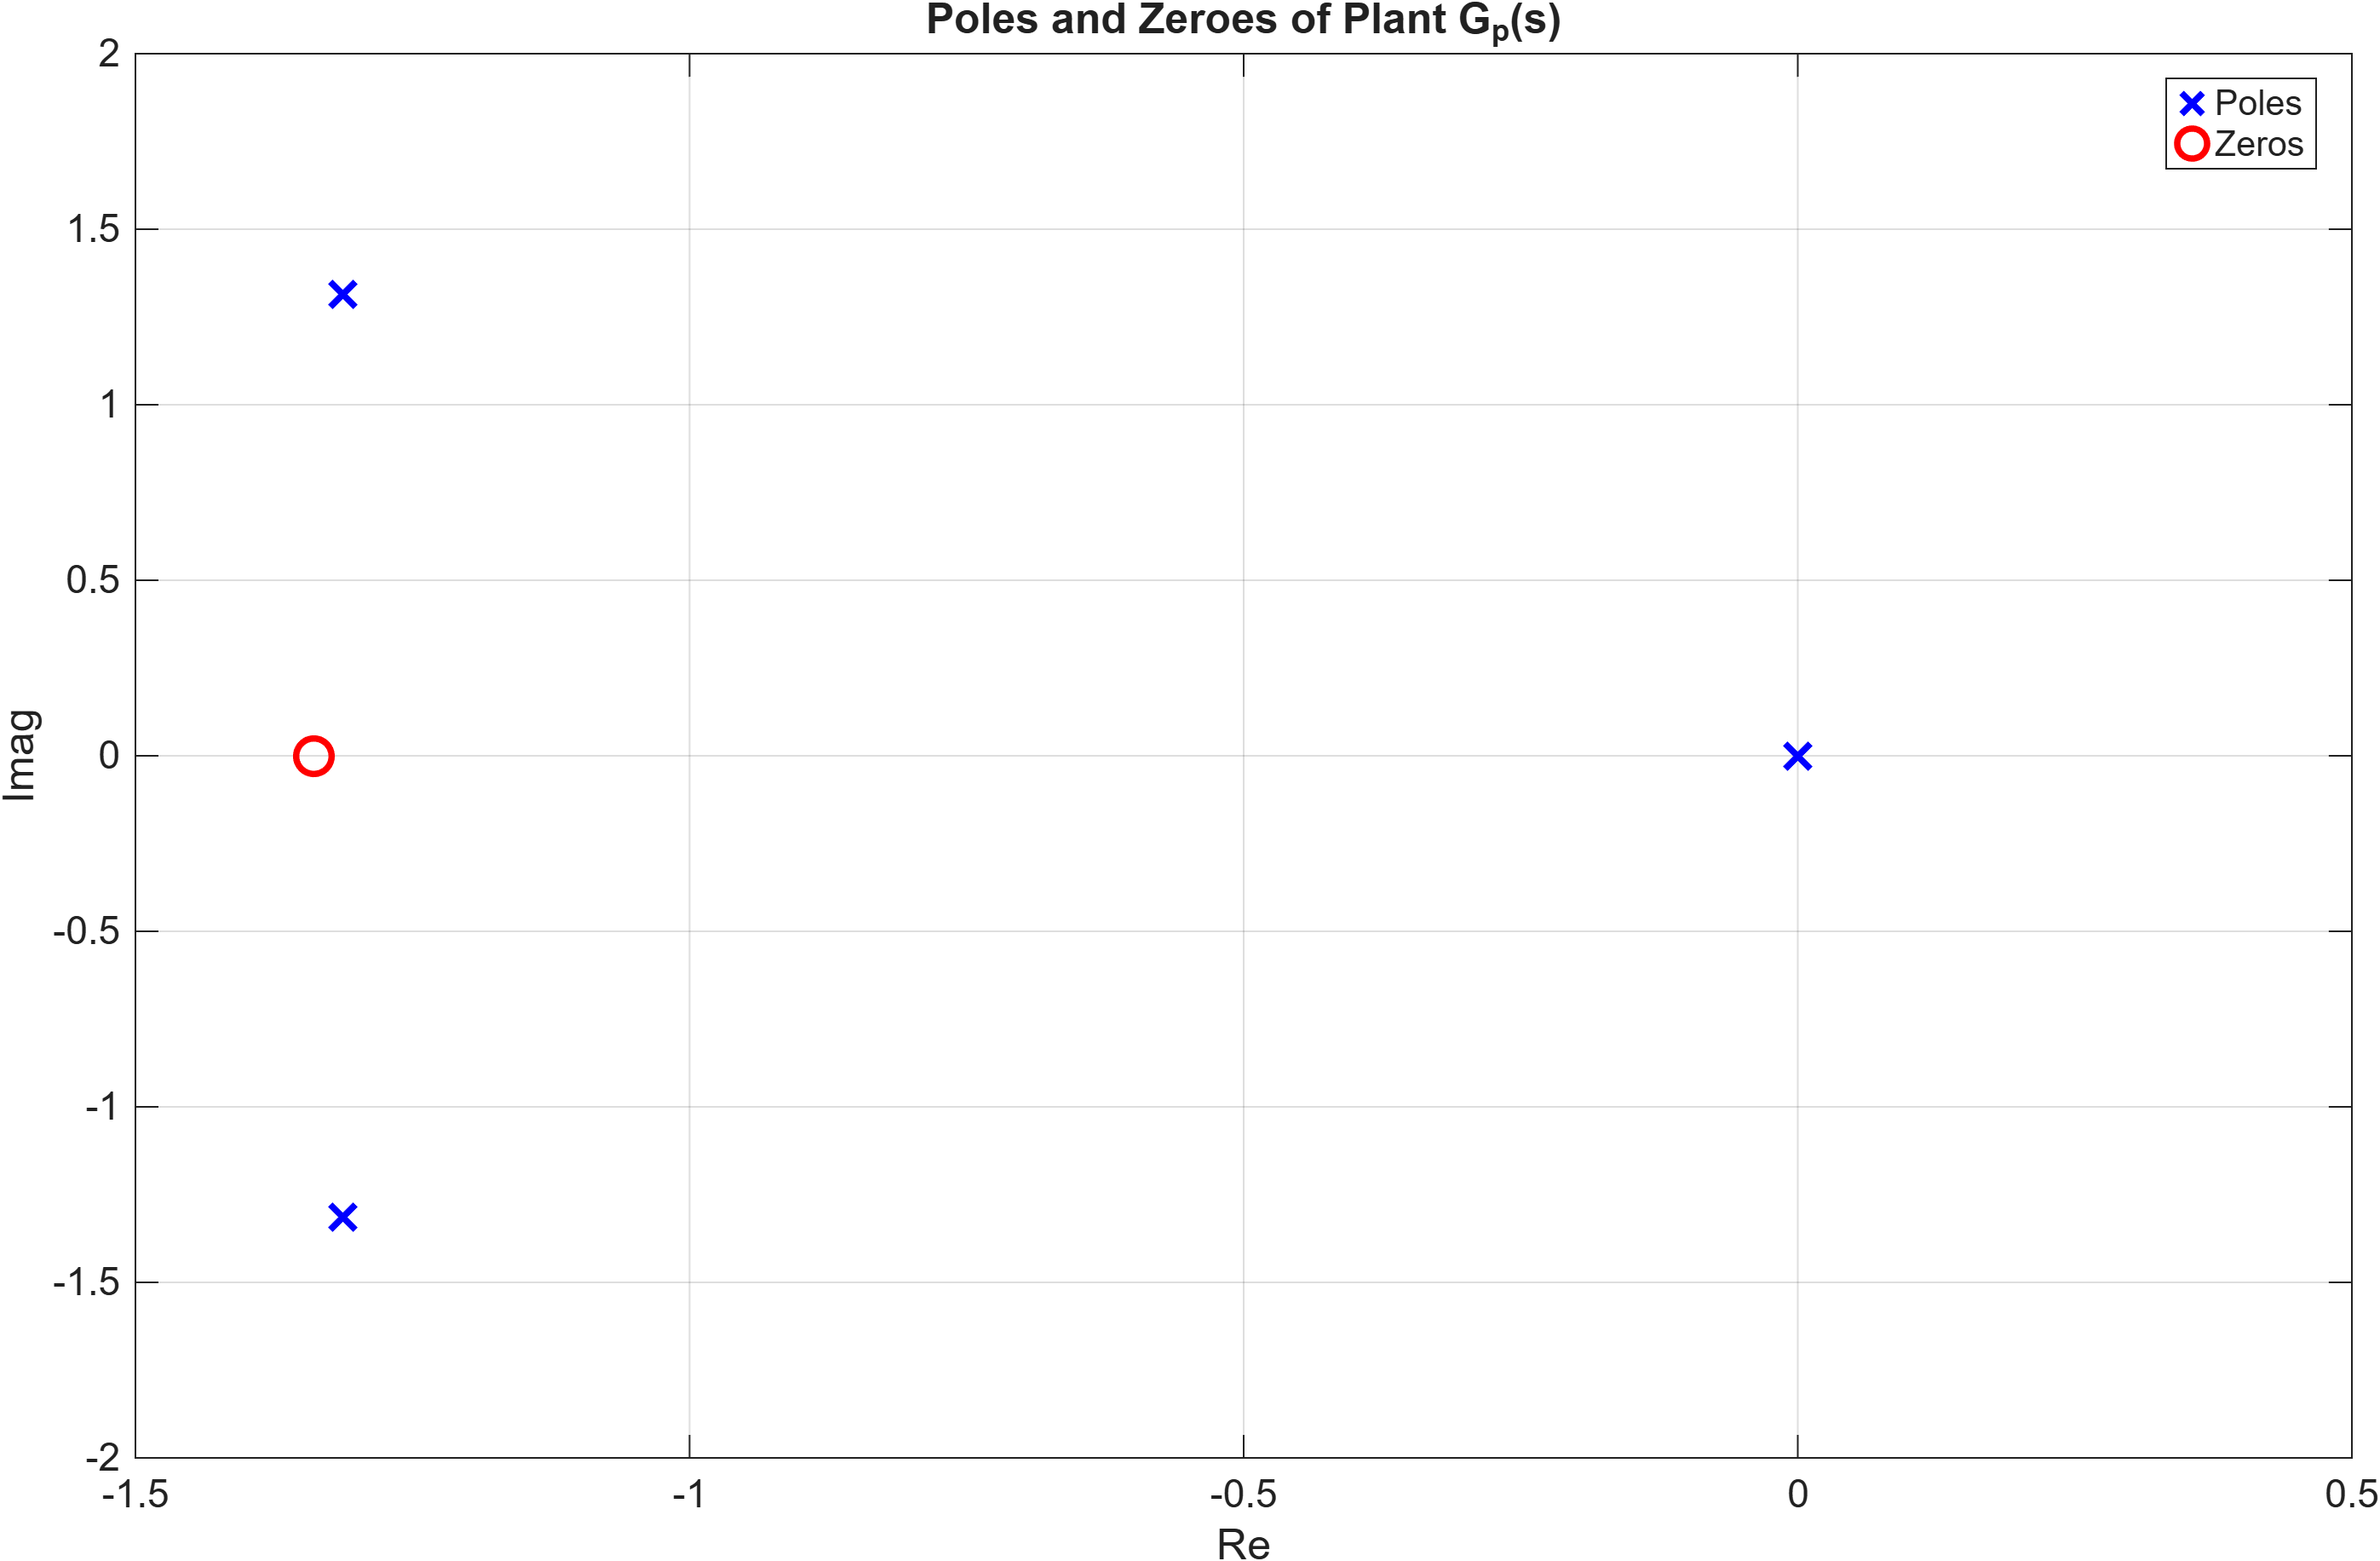
\includegraphics[width=0.8\textwidth]{images/prob1_poleszeros.png}
    \caption{Poles and Zeroes of the Plant described by~\eqref{eq:g_p(s)}}
\end{figure}
The time constant of the real, negative zero $z_1$ is given by $\tau_{z_1} = 1/1.34 = 0.746$s.
\subsection{Control Design Specification}
The specification for the control design are detailed as:
\begin{enumerate}[label=\roman*., ref=\thesubsection(\roman*)]
    \item 
    The resulting closed-loop system is stable. This can be verified
    (not proven) by showing that the real components of all the
    closed-loop system poles are negative.
    \label{spec:stability}

    \item 
    There is zero steady-state error to a step input. This is realised
    by ensuring that the DC gain of the closed-loop system should equal 1.
    \label{spec:sse}

    \item 
    The 2\% settling time of the system does not exceed $1.492$ s,
    and is not less than $0.249$ s.
    \label{spec:settling}

    \item 
    The PO\% does not exceed 80\% of the PO\% of a canonical second-order
    system whose poles equal
    $s_i, s_j = -1.31 \pm j1.32$, or does not exceed 30\%, whichever of
    these constraints is larger.
    \label{spec:overshoot}
\end{enumerate}

This equated to a unity negative feedback control system, with plant modelled by transfer function $G_p(s)$ and controller modelled by transfer function $G_c(s)$. The equivalent closed loop transfer function will equal:
\begin{equation}
G_{cl}(S)=\frac{G_C(s)G_P(s)}{1+G_C(s)G_P(s)}.
\label{eq:g_cl_general}
\end{equation}

The second order canonical system described in this constraint is modelled as having damping ratio $\zeta$ described by: 
\begin{align*}
    &\frac{1.32}{1.31} = \frac{\sqrt{1 - \zeta^2}}{\zeta} \\
    \implies &\zeta \approx \sqrt{\frac{1}{2.02}} = 0.703
\end{align*}
The formula for percentage overshoot of a second order canonical system can then be applied to find the percentage overshoot target for the control design in question:
$$
    \text{PO\%} = 0.8\bigg(100 \exp \big(-\frac{0.703 \pi}{\sqrt{(1 - 0.703^2)}} \big) \bigg) = 3.58\%
$$
The constraint of percentage overshoot not exceeding 30\% will be used for this control design.
\subsection{Topology Discovery}
The control system is implemented using a unity negative-feedback configuration. The reference input \(R(s)\) represents the desired value for the pitch-angle deviation, while \(\tilde{\Theta}(s)\) represents the actual pitch-angle deviation. The controller \(G_c(s)\) operates on the error \(E(s)=R(s)-\tilde{\Theta}(s)\), generating the elevator input according to \(\tilde{\Delta}_e(s)=G_c(s)E(s)\). The resulting closed-loop reference-to-output transfer function, neglecting disturbances, is therefore

$$
T(s)=\frac{\tilde{\Theta}(s)}{R(s)}
=\frac{G_c(s)G_p(s)}{1+G_c(s)G_p(s)}.
$$

Specification~\ref{spec:sse} requires that the open-loop system should have a pole present at $s=0$. This pole is provided by the plant, so the specification is met without the insertion of an I-term at the controller.

Specification~\ref{spec:settling} implies that the dominant poles of the closed loop transfer should be placed to the left of $\approx 4/1.492s$, and to the right of $\approx 4/0.249s$ i.e. $-16.06\le \Re(s) \le  -2.68$. 

The overshoot constraint will be met by the closed loop system having a dominant real pole, or the closed loop system being dominated by a pair of conjugate poles with a sufficiently high damping ratio.

As the plant provides a pole at zero, providing a DC gain of 1, there is no need to insert an I-term to the controller. As derivative components can be difficult to realise, the topology of a P controller should first be investigated.

The root loci of the closed loop system with a P controller are found to have two asymptotes, approaching at $\pi/2$ and $3\pi/2$. These asymptotes approach a value of $\sigma = \frac{0 + 2(-1.31) - (-1.34)}{2} \approx -0.64$. The root loci can then be sketched:

\begin{figure}[H]
    \centering
    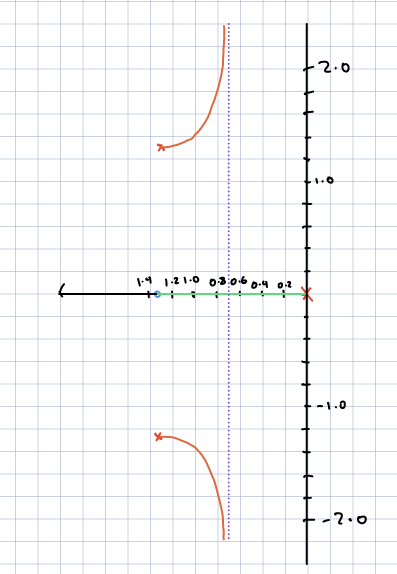
\includegraphics[width=0.8\linewidth,height=0.35\textheight,keepaspectratio]{images/prob1_pcontrol_rootlocus.png}
    \caption{Root Loci of Control Design with P-Controller}
    \label{fig:prob1_pcontrol_rootlocus}
\end{figure}

From these, it is evident that a P controller will not be sufficient. No value of K will place a closed loop pole on any of the sketched loci that will meet the timing constraints of the control system. The three root loci are not sufficiently negative to meet the settling time constraint. 

A practical PD controller is the next logical topology to investigate. The derivative action introduces a controller zero at $s=-z$, allowing the root locus to be reshaped to achieve the desired closed-loop pole locations. An additional pole at $s=-p$ is introduced through a first-order low-pass filter, limiting the controller's high-frequency gain and ensuring that it remains realisable. $p$ and $z$ are chosen such that a pole with a sufficiently negative real component to meet the timing restraints can be found, while also ensuring the poles that lie on the asymptotic loci have a sufficiently high damping ratio to meet the overshoot constraint.

The closed loop system will have four poles; one on the root locus between $0$ and $-1.34$, one on the root locus between $-z$ and $-p$, and a complex conjugate pair of poles on the asymptotic loci. The pole on this rightmost locus will likely dominate the response of the closed loop system as it will be closest to the imaginary axis; this is undesirable as this pole is not negative enough to meet the timing constraints of the control design. The design goal here is to:
\begin{itemize}
    \item Ensure that this "slow" pole on the rightmost root locus is not able to dominate the response, by placing it sufficiently close to the zero at $-1.34$ while keeping a reasonable gain value.
    \item Ensure that the real pole on the root locus between $-z$ and $-p$ is sufficiently negative to meet the settling time constraint.
    \item Ensure that the conjugate poles are sufficiently negative to not disturb the dominance of the real pole between $-z$ and $-p$, and have a damping ratio sufficient to meet the overshoot constraints. 
\end{itemize}
The 30\% overshoot limit gives relative flexibility in the damping ratio constraint. If the conjugate poles have a sufficiently large magnitude, the transient response will initially be dominated by these poles, which can be modelled as an approximate second-order system. Applying the approximate second-order model for the damping ratio of these poles:
$$
\exp \big(-\frac{\pi \zeta}{\sqrt{1 - \zeta^2}} \big ) \le 0.3 \implies \zeta \ge 0.36 
$$
$\zeta=0.36$ gives a very approximate guideline for the damping ratio that will give sufficiently low overshoot; the system in question here does not follow this second order model, so a damping ratio of this value will likely not give a sufficiently low overshoot, but it acts as a suitable design guide. 

If the real part of these conjugate poles are sufficiently negative relative to the real pole on the root locus between $z$ and $p$, their transient response will decay at a much faster rate, leaving the response dominated by that real pole. 

The zero of the controller should be placed sufficiently negative, such that the pole on this locus will be negative enough to meet the timing constraint. The zero should also be sufficiently far enough away from the resulting zero, so that it does not damp the dominance of that pole. A value of $z=2.5$ is chosen initially as a rough estimate of a suitable value.

The PD controller design can be approximated by sketching some topologies with $z=2.5$ and varying $p$:
\begin{figure}[H]
    \centering
    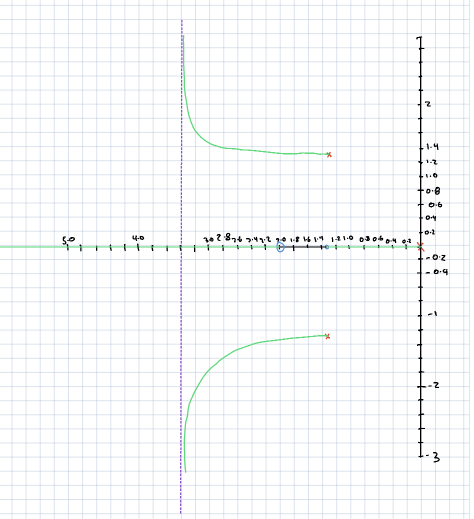
\includegraphics[width=0.85\linewidth,height=0.32\textheight,keepaspectratio]{images/prob1_pdcontrol_p8.png}
    \caption{Root Locus for Controller Pole at $p=8$, two loci approaching $\sigma = -3.39$}
    \label{fig:prob1_pdcontrol_p8}
\end{figure}
\begin{figure}[H]
    \centering
    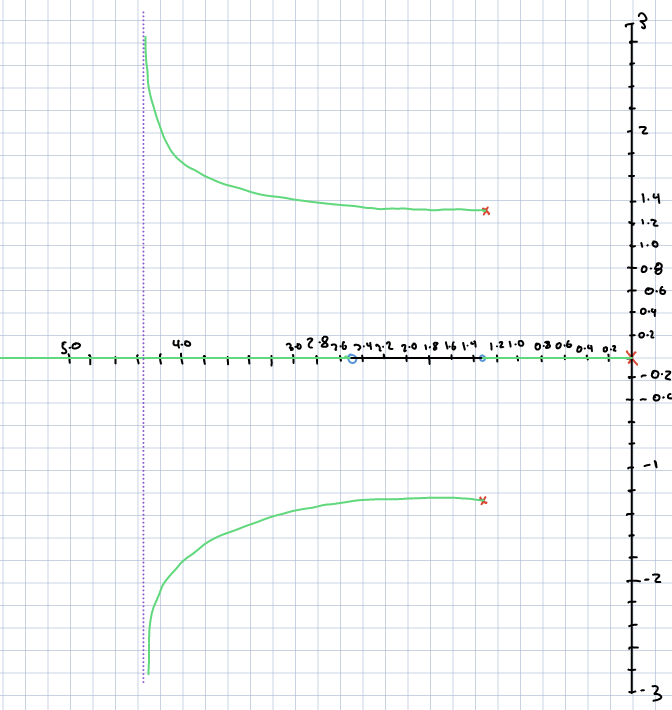
\includegraphics[width=0.85\linewidth,height=0.32\textheight,keepaspectratio]{images/prob1_pdcontrol_p10.png}
    \caption{Root Locus for Controller Pole at $p=10$, two loci approaching $\sigma = -4.39$}
    \label{fig:prob1_pdcontrol_p10}
\end{figure}
\begin{figure}[H]
    \centering
    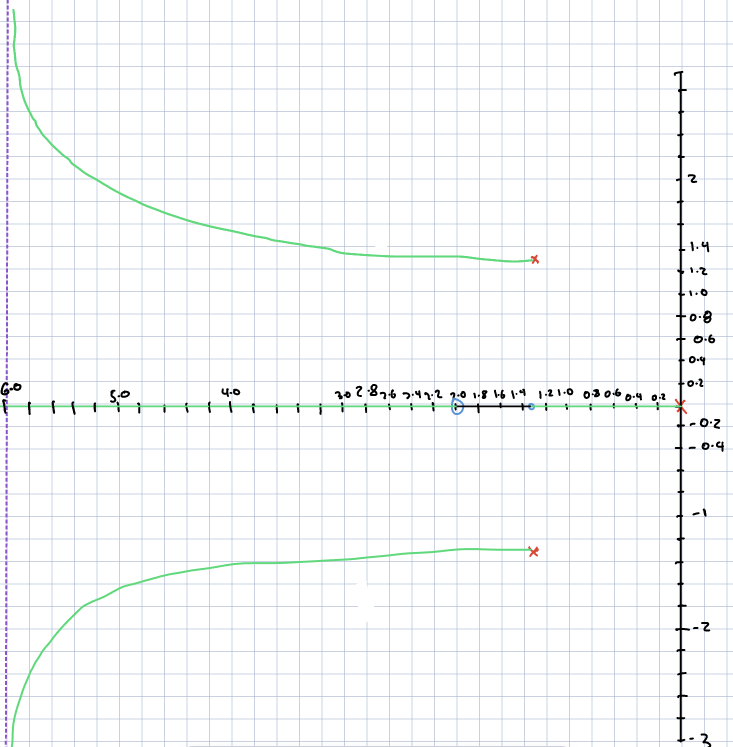
\includegraphics[width=0.85\linewidth,height=0.32\textheight,keepaspectratio]{images/prob1_pdcontrol_p15.png}
    \caption{Root Locus for Controller Pole at $p=13$, two loci approaching $\sigma = -5.89$}
    \label{fig:prob1_pdcontrol_p15}
\end{figure}
$p=10$ appears to be a suitable approximate value; poles less negative than $s=-10$ appear to require significantly large gain values in order to make the complex conjugate poles sufficiently negative. These poles will also have lower damping ratios, and may struggle to reach the overshoot requirement. Poles more negative than $s=-10$ appear to create loci that will be suitable for pole placement that will meet the specification, but these will require larger gain values to realise poles that can be more easily replicated with smaller controller poles. These more negative poles will also require a much smaller $T_d$ for the practical PD controller implementation, which is more difficult to realise.

The sketching process shows that a PD controller with zeros and poles at $z=2.5$ and $p=10$ appears to be a suitable candidate for this control problem. An acceptable approximation of the placement of the real closed loop pole can be made around $s\approx -3$, to provide the required component for settling time. Assuming that the rightmost pole is sufficiently close to the plant zero such that it's influence on the transient response is negligible, and assuming that the complex conjugate poles are sufficiently more negative than $-3$, the 2\% settling time of the system can be roughly approximated using a first order model, $T_s \approx\frac{4}{3s^{-1}}\approx1.33s$. This satisfies the settling time requirement.

These can be further investigated via numerical analysis in Matlab, making use of the \texttt{rlocfind} function. The \texttt{rlocfind} command is used to plot the root loci, and a pole with a sufficiently negative real component of $p \approx -3$ is placed on the real axis. 

The resulting complex conjugate pair of poles must be suitably damped, and the resulting rightmost pole must be sufficiently close to the plant zero to allow the dominance of the more negative pole. 

The \texttt{rlocfind} defines the closed loop poles of the system as below:
\begin{figure}[H]
    \centering
    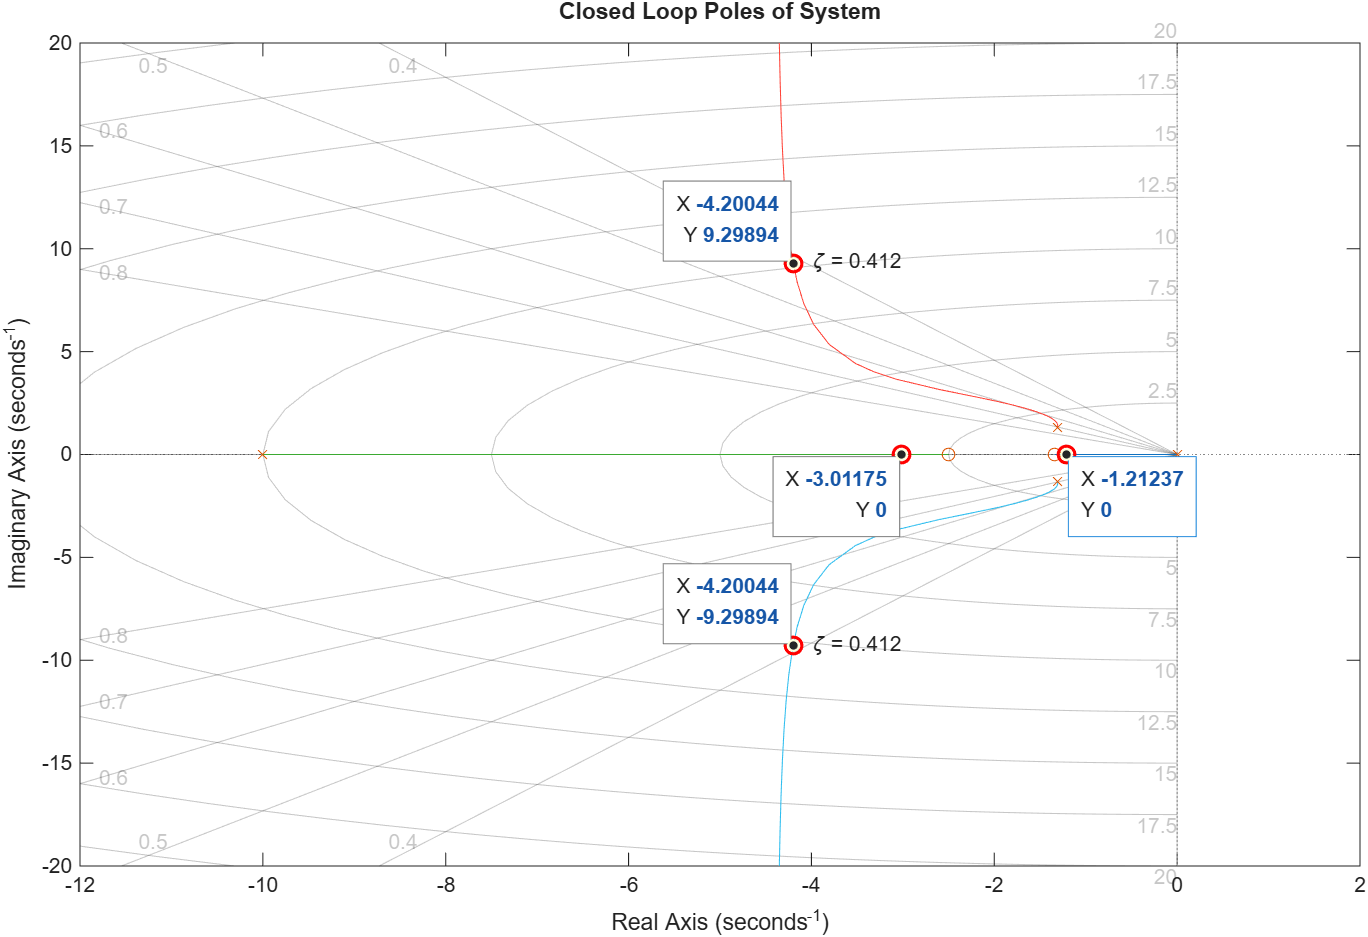
\includegraphics[width=0.8\linewidth]{images/prob1_pdcontrol_matlab_pole3.png}
    \caption{Closed loop poles for system, found using \texttt{rlocfind}}
    \label{fig:prob1_pdcontrol_matlab_pole3}
\end{figure}

A gain value of $K = 84.019$ is required to realise this closed loop system, i.e. the basic controller form is of the following:
$$
G_c(s) = 84.019\frac{s + 2.5}{s+10} = \frac{8.4019s+21.00475}{0.1s+1}
$$

The closed loop system has poles at the following locations:
\begin{align*}
    p_{cl, 1} &= -1.21 + j0 \\
    p_{cl, 2} &= -3 + j0 \\
    p_{cl, 3} &= -4.2 + j9.3 \\ 
    p_{cl, 4} &= -4.2 - j9.3 \\ 
\end{align*}
The rightmost pole $p_{cl, 1}$ lies close to the plant zero at $-1.34$, and as such will likely struggle to dominate the response of the system. The response will be dominated by the remaining poles; as the real component of $p_{cl, 2}$ is less negative than those of $p_{cl, 3}, p_{cl, 4}$, this pole will dominate the transient system response, and is sufficiently negative to meet the timing constraint as estimated by the first order model. As the dominance of $p_{cl, 2}$ is being established, the complex conjugate pair will have a non-neglible contribution, so overshoot will occur. Matlab provides a damping ratio for these poles of $\zeta = 0.412$, which is greater than the minimum $\zeta_{min} = 0.36$ that the approximate second-order model estimates.

Thus, the derived PD controller can be defined in standard format:
\begin{equation}
    G_c(s) \approx \underbrace{21}_{k_p} + \underbrace{6.3}_{k_d}\frac{s}{\underbrace{0.1}_{T_d}s + 1}
    \label{eq:prob1_pdcontrol}
\end{equation}

The P and D gain values $k_p$ and $k_d$ are not exceedingly large or small, meaning they could be more easily realised in electronic components if this controller were to be implemented. The time constant $T_d$ is also not excessively small, meaning it would be more easily realised in an implementation of this controller. 

The adherence of the system to the specification can be tested using Matlab. The closed loop system of~\eqref{eq:g_p(s)} controlled by the PD controller described by~\eqref{eq:prob1_pdcontrol} is tested with a step input, using the \texttt{step} and \texttt{stepinfo} commands in Matlab (see Listing~\ref{lst:prob1_stepinfo}).

The step response of the closed loop system can be visualised using the \texttt{step} command:
\begin{figure}[H]
    \centering
    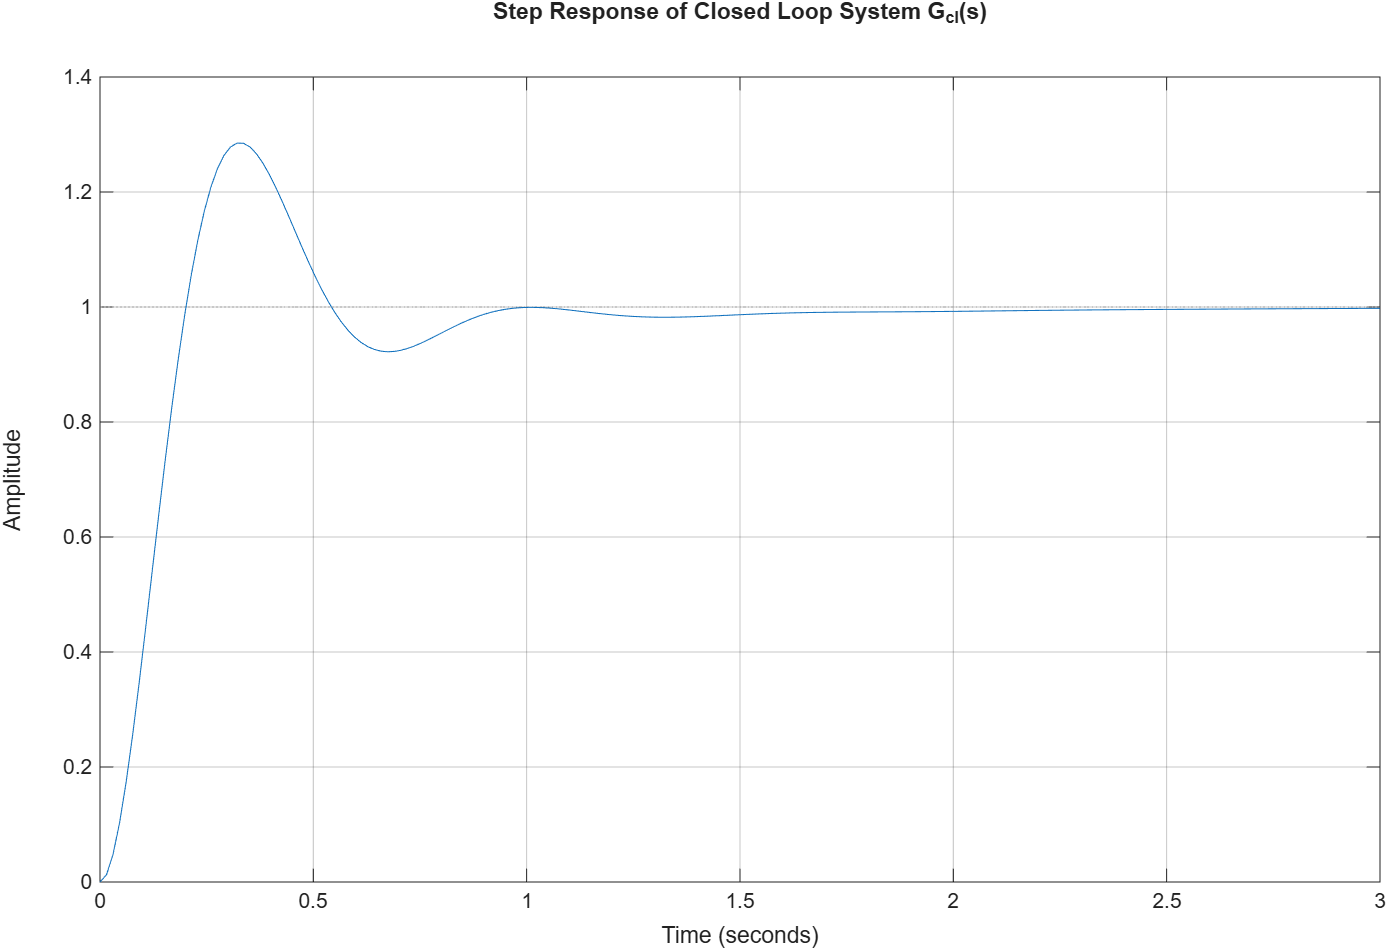
\includegraphics[width=0.8\linewidth]{images/prob1_pdcontrol_matlab_step.png}
    \caption{Closed loop poles for system, found using \texttt{rlocfind}}
    \label{fig:prob1_pdcontrol_matlab_step}
\end{figure}

The adherence to the specification can also be confirmed using the \texttt{stepinfo}, \texttt{isstable} and \texttt{dcgain} commands:
\par\noindent\begin{minipage}{\linewidth}
\begin{lstlisting}[style=outputstyle]
--- Specification checks ---
Stable: True
DC gain: 1.0000
Settling time: 0.8725 s
Overshoot: 28.50 %
\end{lstlisting}
\end{minipage}\par

These results indicate that this closed loop system has achieved the design specification in the ideal simulation environment. 

\subsection{Disturbance Rejection}
To characterise the disturbance rejection performance of the closed loop system derived above, the transfer function for disturbance must be defined.

As the coefficients of the elevator input \(\tilde{\delta}_e\) and disturbance \(d\) are identical in both~\eqref{eq:atild} and~\eqref{eq:qtild}, these inputs have an identical effect on the plant. By linearity, the previously derived plant transfer function~\eqref{eq:g_p(s)} can therefore be used to describe the response to their combined input:

\[
\tilde{\Theta}(s)=G_p(s)\left[\tilde{\Delta}_e(s)+D(s)\right].
\]

The closed loop system can then be derived. As stated earlier, the error in this closed loop system is given by:
$$
E(s) = R(s) - \tilde{\Theta}(s)
$$
Assuming the reference signal $R(s)$ is set to 0, the error is simplified to $E(s) = - \tilde{\Theta}(s)$. The corresponding elevator pitch setting $\tilde{\Delta_e}(s)$ is then found as:
$$\tilde{\Delta_e}(s) = -G_c(s)\tilde{\Theta}(s)$$

This yields a model for the closed-loop system's reaction to a disturbance input:
\begin{align*}
\tilde{\Theta}(s) &=G_p(s)\left[\tilde{\Delta}_e(s)+D(s)\right] \\
&= G_p(s)\left[-G_c(s)\tilde{\Theta}(s) + D(s)\right] \\
\tilde{\Theta}(s) \left[1 + G_C(s)G_p(s) \right] &= G_p(s) D(s)
\end{align*}
The closed loop transfer function can then be defined:
\begin{equation}
\frac{\tilde{\Theta}(s)}{D(s)}
=\frac{G_p(s)}{1+G_c(s)G_p(s)}
\label{eq:prob1_disturbance}
\end{equation}  
The response of this closed loop system to an impulse response can be completed using Matlab's \texttt{impulse} command. This passes a unit-area impulse as input to a system modelled by a transfer function. 

The disturbance rejection can be tested by passing a unit area impulse signal $d(t) = \delta(t)$, where $\delta(t)$ is the Dirac delta function. This will yield an impulse response \textit{per unit impulse area}. 

\begin{figure}[H]
    \centering
    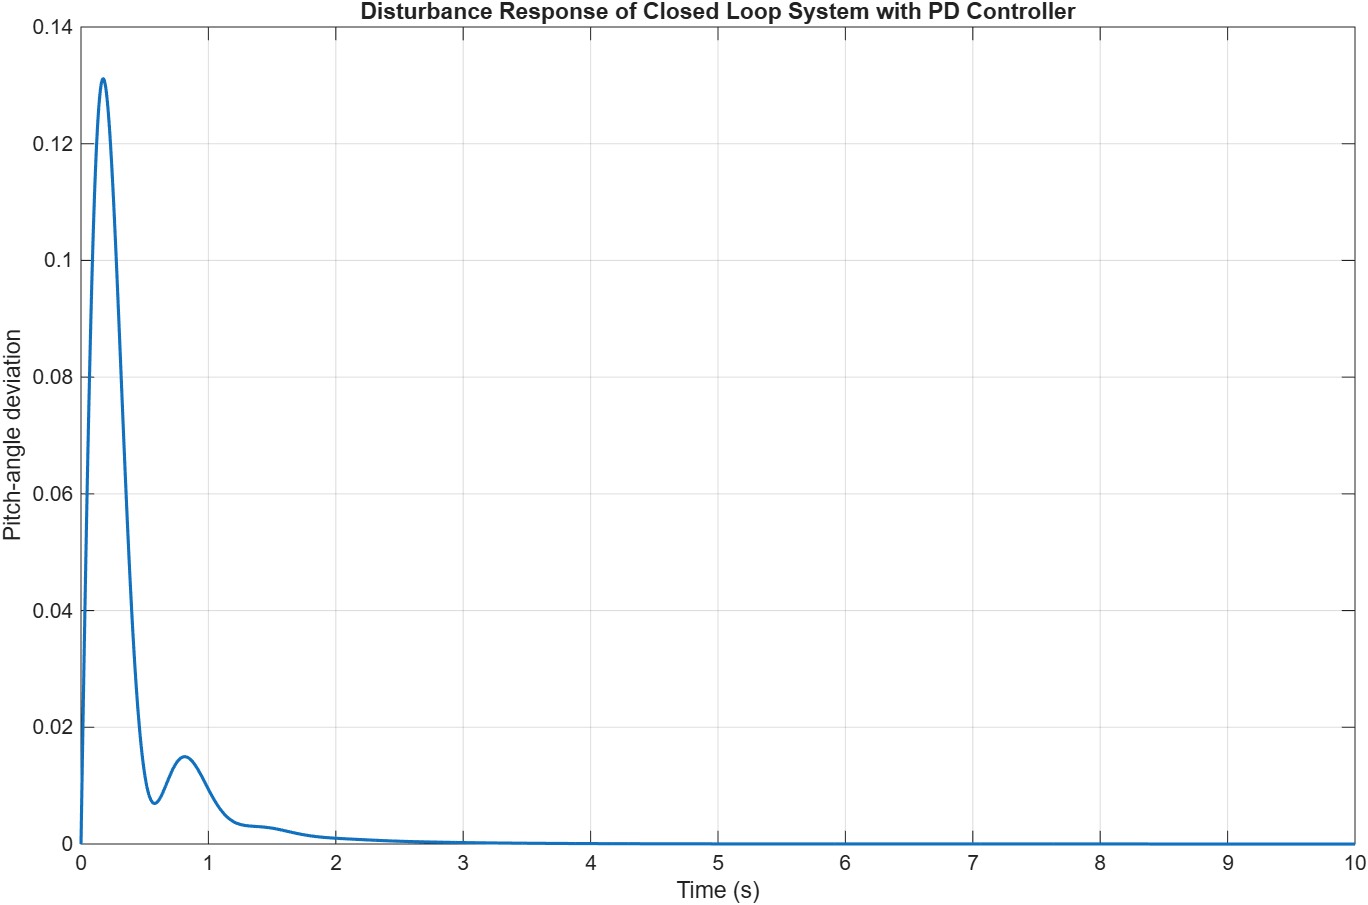
\includegraphics[width=0.8\textwidth]{images/prob1_pdcontrol_matlab_impulse_cl.png}
    \caption{Impulse response of closed loop system described by~\eqref{eq:prob1_disturbance}}
\end{figure}

The impulse response of the closed-loop system indicates satisfactory disturbance rejection. The maximum absolute pitch-angle deviation resulting from a unit-area impulsive disturbance is \(\max_{t\geq 0}|\tilde{\theta}(t)| = 0.13112\) angle units. The response is shown to fall to less than $2\%$ of this maximum deviation within 1.523 seconds. 

This disturbance rejection can also also shown to be asymptotically stable using the $\texttt{isstable}$ command in Matlab. This is the expected behaviour of the system, as governed by the Final Value Theorem. To show this, the following re-arrangement can be made:

\begin{align*}
    G_d(s) &= \frac{\tilde{\Theta}(s)}{\underbrace{D(s)}_{1}} = \frac{G(s)}{1+G(s)G_C(s)} \\
    \implies \tilde{\Theta}(s) &= G_d(s)
\end{align*}

Applying the Final Value Theorem:
\[
    \lim_{t\to\infty}\tilde{\theta}(t) = \lim_{s\to0}sG_d(s)
\]
As $G_d(s)$ has poles with poles strictly less than 0, the above limit will tend to 0. 

This demonstrates that the closed-loop system rejects the impulsive disturbance without a persistent deviation from the equilibrium operating point.

\subsection{Control Design Robustness}
To measure the robustness of the control design to plant modelling errors, a Matlab script can be used to vary the $a_{11}$ and $a_{21}$ parameters, introducing an error of up to 10\% on both coefficients. This script sweeps across 21 equally spaced errors between $\pm10\%$ for both coefficients, totalling 441 total simulations of step response (see Listing~\ref{lst:prob1_err}). 

The two specifications of concern for an incorrectly modelled plant are~\ref{spec:settling} and~\ref{spec:overshoot}. Across all 441 simulations, the system stays within the bounds of settling time and overshoot defined by the specifications:
\par\noindent\begin{minipage}{\linewidth}
\begin{lstlisting}[style=outputstyle]
    Settling time:  0.860 to 1.411 s
    Overshoot:      28.27 to 28.75 % 
\end{lstlisting}
\end{minipage}\par
The system can be estimated as robust to errors up to $\pm10\%$ in the estimation of the two analysed coefficients.


\subsection{Stability Robustness}
A similar analysis can be performed for the robustness of the stability of this closed loop system. A similar Matlab script can be used to introduce an error of up to $\pm10\%$ on the two co-efficients (see Listing~\ref{lst:prob1_staberr}). The stability of the system can be quantified by looking at the corresponding system poles, and verifying that these poles do not cross the imaginary axis.

Stability is observed across all 441 simulated parameter combinations. The closed-loop pole with the largest real component, corresponding to the configuration closest to instability, occurred when \(a_{11}\) was 10\% below its nominal value and \(a_{21}\) was 10\% above its nominal value. The rightmost closed-loop pole had a real component of \(-1.0955\), remaining strictly within the left half of the complex plane. These results provide strong numerical evidence that the designed controller is robustly stable under the specified \(\pm 10\%\) parameter uncertainties.

\clearpage
\section{Problem 2}
Upon substitution of the personalised digits, the following ODE describing a SISO plant can be defined: 
\begin{equation}
    f(t) = \ddot{x} - \left( 1.52 - 0.507 x^2 \right) \dot{x} + 1.5x + 0.04x^3 + 0.07x^5
    \label{eq:prob2_ode}
\end{equation}

\subsection{System Oscillatory Behaviour}
The special condition of setting this equation to equal 0 yields an ODE that can be analysed numerically in Matlab. This can be analysed using the \texttt{ode45} method to solve the ODE using the RK45 method.~\cite{mathworks:ode45}

A set of initial conditions must first be defined, $x = 1, \dot{x} = 0$ is a suitable arbitrary choice to view the convergence to a limit cycle. 

\begin{figure}[H]
    \centering
    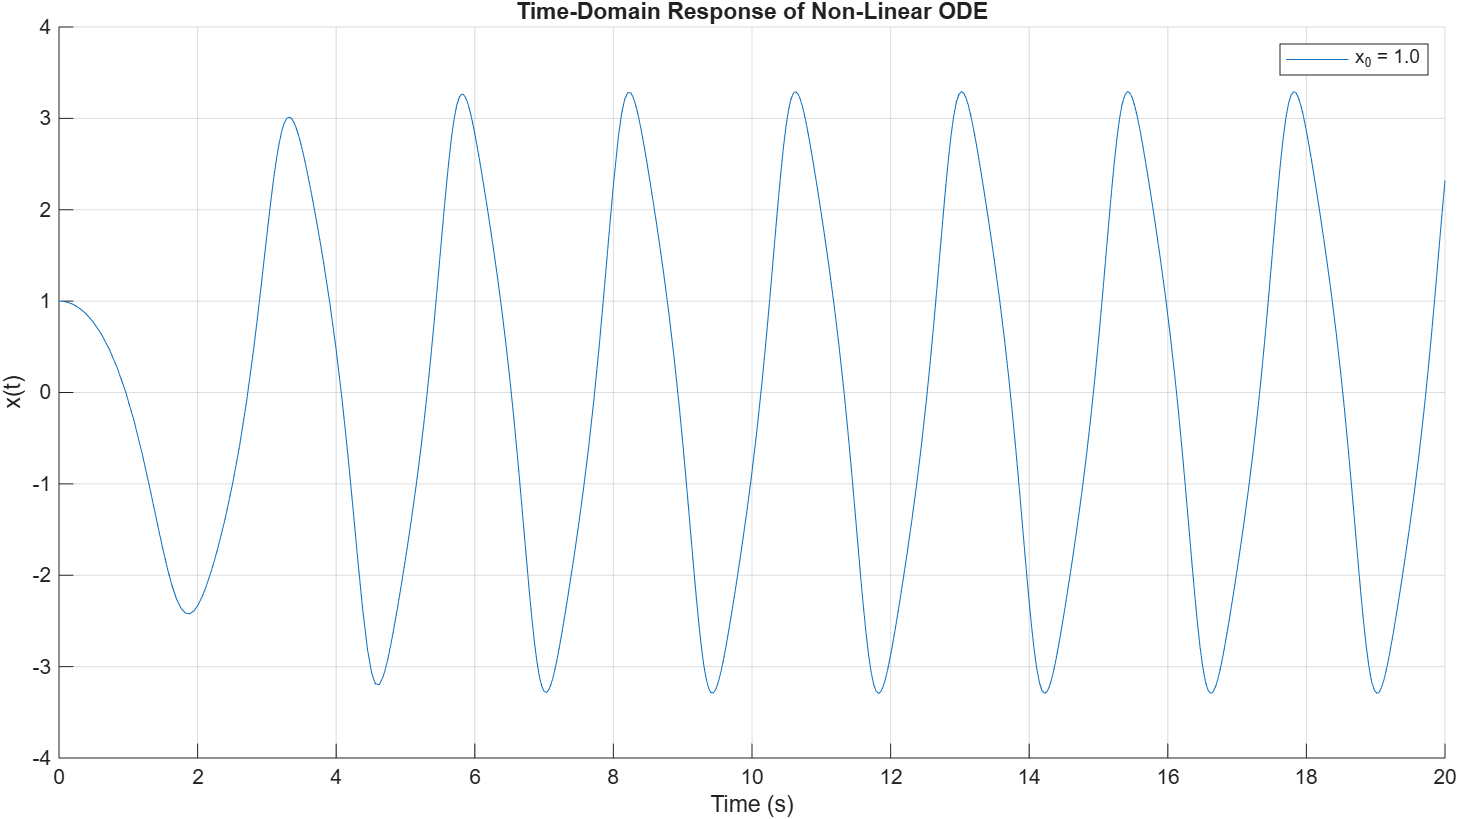
\includegraphics[width=0.95\textwidth]{images/prob2_odelimitcycle_x1.png}
    \caption{Time-domain response of system described by~\eqref{eq:prob2_ode} $= 0$, $x=1, \dot{x}=0$}
\end{figure}
With this set of initial conditions, the equation appears to converge towards an oscillation of amplitude $A \approx 3.29$. To investigate other initial conditions and their oscillatory behaviour, a range of initial conditions can be defined: 
\[
\begin{bmatrix}
x(0) & \dot{x}(0)
\end{bmatrix}
\in
\left\{
    \underbrace{
        \begin{bmatrix} 0.5 & 0 \end{bmatrix},
        \begin{bmatrix} 3.29 & 0 \end{bmatrix}
        \begin{bmatrix} 5.0 & 0 \end{bmatrix},
    }_{\text{Varying }x(0)}
    \underbrace{
        \begin{bmatrix} 0 & 1 \end{bmatrix},
        \begin{bmatrix} 0 & 8 \end{bmatrix},
    }_{\text{Varying }\dot{x}(0)}
\right\}.
\]

These initial conditions seek to observe how the convergence of this special condition to a limit cycle changes, depending on how $x$ and $\dot{x}$ are varied. 

These initial conditions are evaluated using \texttt{ode45} and plotted:
\begin{figure}[H]
    \centering
    \begin{subfigure}[t]{0.75\textwidth}
        \centering
        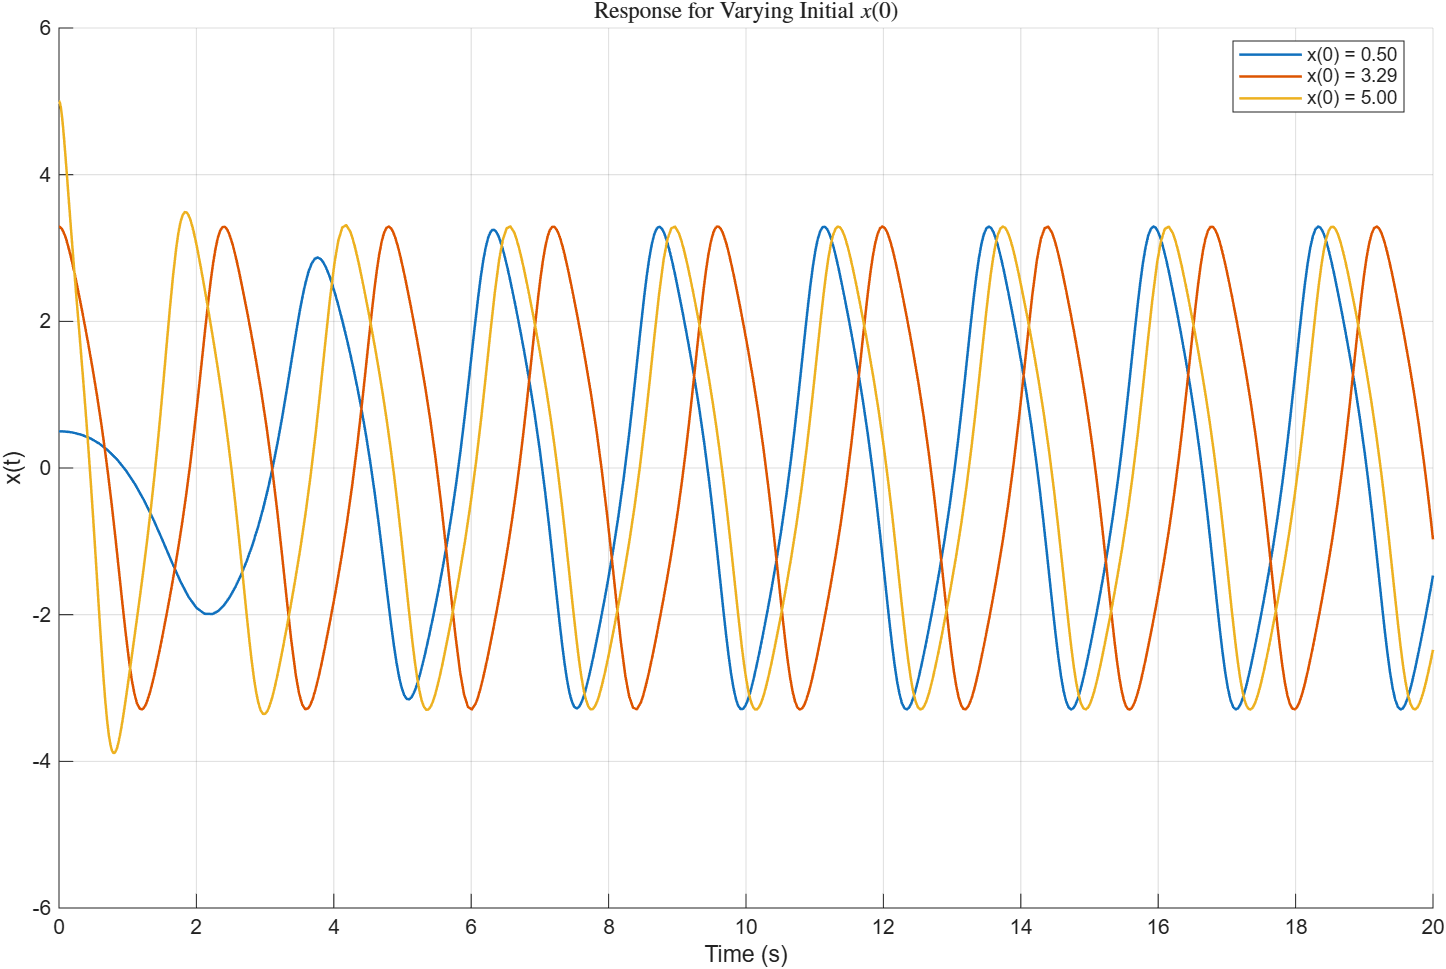
\includegraphics[width=\linewidth]{images/prob2_odelimitcycle_varx.png}
        \caption{Varying initial displacement $x(0)$}
        \label{fig:limitcycle_x}
    \end{subfigure}
    \hfill
    \begin{subfigure}[t]{0.75\textwidth}
        \centering
        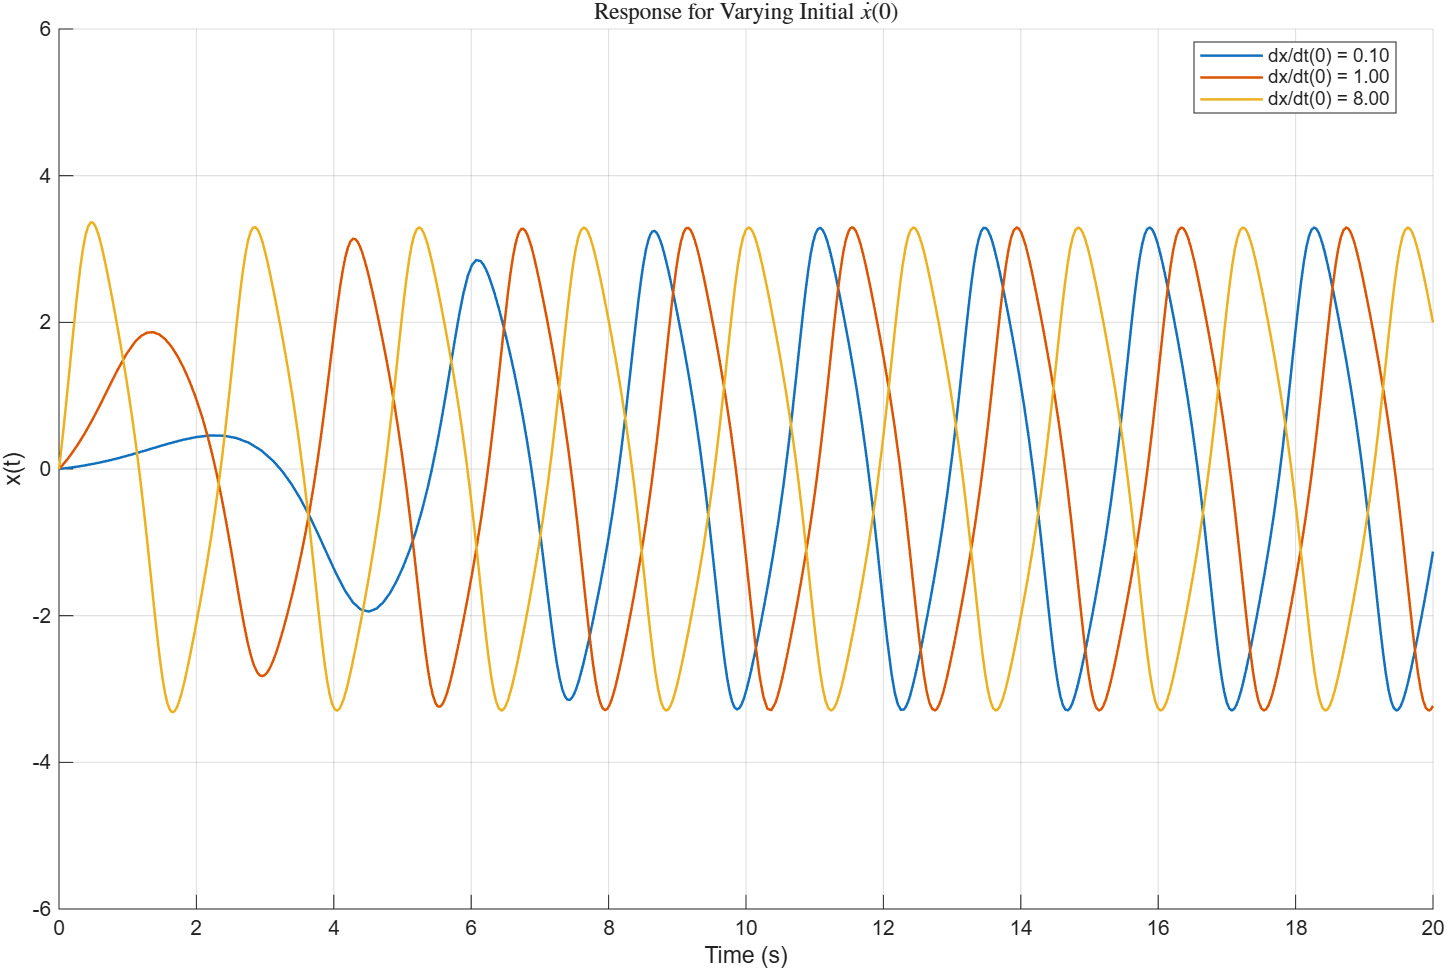
\includegraphics[width=\linewidth]{images/prob2_odelimitcycle_vardotx.png}
        \caption{Varying initial velocity $\dot{x}(0)$}
        \label{fig:limitcycle_xdot}
    \end{subfigure}
    \caption{Time-domain responses of the nonlinear oscillator for different initial conditions.}
    \label{fig:limitcycle}
\end{figure}
As can be observed in these plots, the non-linear ODE appears to converge to a stable oscillation, across a range of initial conditions. The initial amplitude of the limit cycle appears to be related to $x$, and the speed of convergence to a limit cycle appears to be governed by $\dot{x}$.

This oscillation can be quantified by finding it's peak values and frequency. Across the different initial conditions, a consistent oscillation is found, of amplitude 3.292 and frequency 0.417 Hz. This yields a period of $1/0.417 \approx 2.399s$. 

\subsection{Linearisation}
To linearise the system around the desired operating point of $x = 0, \dot{x} = 0$, a first-order Taylor series can be completed.


The derivative $\ddot{x}$ can be expressed as a function of $x, \dot{x},$ \& $f$:
$$
    \ddot{x} = g(x,\dot{x},f)=(1.52-0.507x^2)\dot{x}-1.5x-0.04x^3-0.07x^5+f
$$

The first-order Taylor expansion for this $g(x, \dot{x}, f)$ at the desired operating point is given as: 

\begin{align*}
g(x,\dot{x},f)\approx {}&
g(x_0,\dot{x}_0,f_0)\\
&+\left.\frac{\partial g}{\partial x}\right|_0(x-x_0)\\
&+\left.\frac{\partial g}{\partial\dot{x}}\right|_0(\dot{x}-\dot{x}_0)\\
&+\left.\frac{\partial g}{\partial f}\right|_0(f-f_0)
\end{align*}

The partial derivaties with respect to the three variables can be found, and evaluated at the operating point:

\begin{align*}
    \left.\frac{\partial g}{\partial x}\right|_{(0,0,0)} &= -1.5 \\
    \left.\frac{\partial g}{\partial \dot{x}}\right|_{(0,0,0)} &= 1.52 \\
    \left.\frac{\partial g}{\partial f}\right|_{(0,0,0)} &= 1 \\
    \implies \ddot{x} &= -1.5x + 1.52\dot{x} + f
\end{align*}

Thus, the linearised approximation of the function $f(x)$ about the operating point $x = 0, \dot{x} = 0$ is given by:

\begin{equation}
    f(t) \approx \ddot{x} - 1.52\dot{x} + 1.5{x}
    \label{eq:prob2_linear}
\end{equation}

The transfer function of~\eqref{eq:prob2_linear} can be found using the Laplace transform. Assuming zero initial conditions, the transform can be performed:
$$
F(s) = s^2X(s) - 1.52sX(s) + 1.5X(s)
$$

This can be re-arranged to give a transfer function in the s-domain for the linearised system: 
\begin{equation}
    G_p(s) = \frac{X(s)}{F(s)} = \frac{1}{s^2 - 1.52s + 1.5}
    \label{eq:prob2_plant_tf}
\end{equation}

The stability of this linearised model can be evaluated by finding the poles of the transfer function via Matlab:

\par\noindent\begin{minipage}{\linewidth}
\begin{lstlisting}[style=outputstyle]
>> Gp = tf([1], [1 -1.52 1.5]);
>> pole(Gp)
    ans = 2x1 complex
        0.7600 + 0.9604i
        0.7600 - 0.9604i
\end{lstlisting}
\end{minipage}\par
As these poles have positive real components, they will create an oscillatory component in the response of this linearised system that grows unbounded over time. As such, the system can be said to be unstable. 

\subsection{Controller Design Specification}
The specifications for the control design are detailed as:
\begin{enumerate}[label=\roman*., ref=\thesubsection(\roman*)]
    \item 
    The resulting closed-loop system is stable. This can be verified as previously.
    \label{spec:stability2}
    \item 
    There is zero steady-state error to a step input. This is realised
    by ensuring that a pole is present in the closed-loop system at $s=0$.
    \label{spec:sse2}
    \item 
    The 2\% settling time of the system does not exceed $0.85\times 2.399s \approx 2.04$ seconds.
    \label{spec:settling2}
    \item 
    The PO\% does not exceed 80\%. This can be estimated with the 2nd order system model to give a minimum damping ratio of $\zeta\geq0.071$.
    \label{spec:overshoot2}
\end{enumerate}

As previously, these specifications translate to a unity negative-feedback control system, with closed loop transfer function~\eqref{eq:g_cl_general}
\subsection{Topology Discovery}
The design of a PID controller can be undertaken to reach these specifications. 

To satisfy Spec~\ref{spec:stability2}, all poles must be in the negative half plane of the real axis, such that their real component is negative. 

Spec~\ref{spec:sse2} requires a pole in the open loop transfer function at $s=0$, to ensure the DC gain of the system equals 1. As there is no pole at the origin in the plant, an $I$ term must be placed in the controller. 

As such, the first topology to be examined will be a PI controller, i.e. a PID controller with zero derivative gain.

\subsubsection{PI Controller Topology}

This controller topology will introduce a gain term, a pole at 0 and one zero. This is equivalent to a controller transfer function $G_c(s) = K_p + \frac{K_i}{s} = \frac{K_ps + K_i}{s}$. 

The feasibility of this topology can be verified via the root locus drawing rules. In this system, there will be three open loop poles and one open loop zero. This will result in $3 - 1 = 2$ asymptotes. They will have centroid $\sigma$ at:
$$
\sigma = \frac{(0+0.76+0.76)-(-z)}{3-1}
=\frac{1.52+z}{2}
$$
The asymptote angles are also found as $\theta_1 = \frac{\pi}{2}, \theta_2 = \frac{3\pi}{2}$. For any $z > 0$ i.e. for positive $K_i$ and $K_p$, no value of $z$ can result in the locus centroid being $< 0.76$. As such, the resulting root locus will never cross the imaginary axis, and as such no gain value can be found to result in the real component of the conjugate pairs to be negative. As such, no PI controller configuration can yield a stable closed-loop system.

\subsubsection{PID Controller Topology}
An ideal implementation of this topology will introduce a gain term, a pole at zero, and two zeros:
$$
G_{C, PID, Ideal} = \frac{k (s + z_1)(s + z_2)}{s}
$$
The practical implementation of a PID controller introduces a small delay constant $T_D$ for numerically stable differentiation; this is chosen as $T_D = 0.1$ in this design as it should be suitably small without being excessively difficult to implement. This yields an additional real pole at $p = -1/0.1 = -10$, giving a controller modelled as:

$$
G_{C,PID}(s)
=k_p+\frac{k_i}{s}+\frac{k_ds}{T_ds+1}
=\frac{K(s+z_1)(s+z_2)}{s(s+10)}
$$

The root locus drawing rules can again be reviewed. The open loop system will have 4 open loop poles and 2 open loop zeroes, resulting in 2 asymptotes. These asymptotes will have centroid $\sigma$ at:

$$
\sigma = \frac{(0 - 10 + 0.76 + 0.76)-(-z_1 - z_2)}{3-1}
=\frac{-8.48 +  z_1 + z_2}{2}
$$
The asymptote angles are $\theta_1 = \frac{\pi}{2}, \theta_2 = \frac{3\pi}{2}$.

This equation assists in the sketching of the root locus. The dominant pole, or pair of conjugate poles, must be negative enough to satisfy the timing constraint. This can be estimated using the approximate model for the settling time of a dominant pole or pair of poles as $
T_s\approx\frac{4}{\operatorname{Re}(p)}\leq2.04
$, i.e. $\operatorname{Re}(p)\leq-1.96$. 

The root loci can be roughly sketched using the drawing rules for varying $z_1, z_2$, to assist in the selection of these values. 

First, a large $z_1$ and $z_2$ are chosen, to determine if a dominant real pole is a feasible topology. This topology seeks to create the rightmost root locus such that a suitably negative real pole can dominate the response.

\begin{figure}[H]
    \centering
    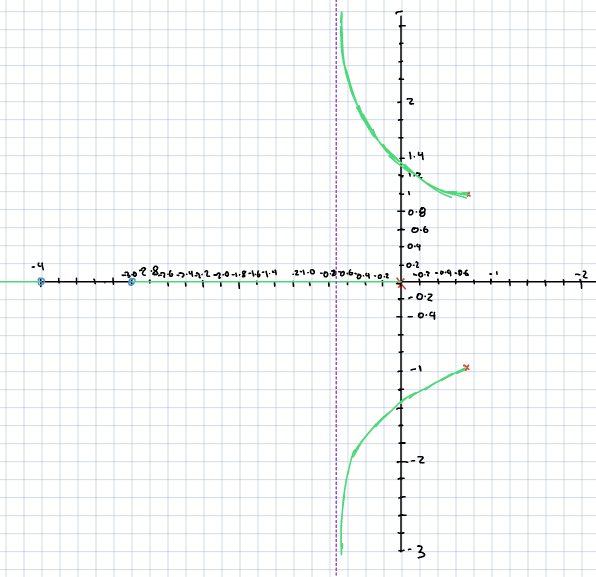
\includegraphics[width=0.8\textwidth]{images/prob2_rootlocussketch_3_4.png}
    \caption{Root Locus Sketch for PID-controlled system, $z_1 = 3, z_2 = 4, p = 10$}
\end{figure}
The sketching of the root locus shows that this is an unsuitable topology. Any value of $K$ will result in a pair of conjugate poles dominating the response, with real part not sufficiently negative to meet the timing requirements. 

As such, the design goal shifts towards a \textit{dominant pair} of poles. For any design utilising $z_1 < 1.96$, the resulting configuration will have a rightmost pole that will fail the timing requirement if it dominates the response; as such, this pole should be placed suitably close to the zero at $z_1$ to prevent it from dominating the response.

$z_1$ and $z_2$ are then made smaller to observe the behaviour of the root locus:
\begin{figure}[H]
    \centering
    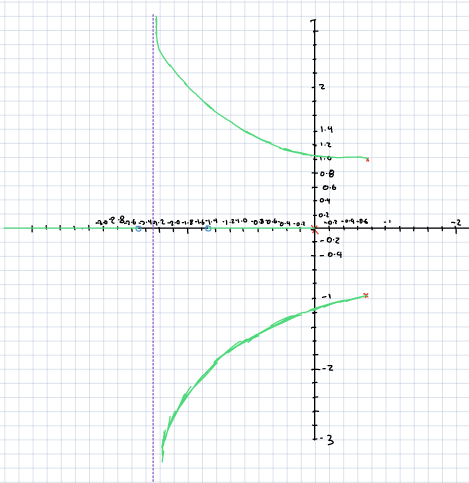
\includegraphics[width=0.8\textwidth]{images/prob2_rootlocussketch_1.5_2.5.png}
    \caption{Root Locus Sketch for PID-controlled system, $z_1 = 1.5, z_2 = 2.5, p = 10$}
\end{figure}

This topology appears to be potentially viable for the specification. A dominant pair of conjugate poles could be placed on the two loci asymptotically approaching $\sigma
=\frac{-8.48 +  1.5 + 2.5}{2} = -2.24$. This could potentially satisfy the timing requirement, however it may require a very large value for gain, and the pole placement may result in the overshoot requirement not being met. 

These concerns are verified using Matlab, and \texttt{rlocfind}:

\begin{figure}[H]
    \centering
    \begin{subfigure}[t]{0.48\textwidth}
        \centering
        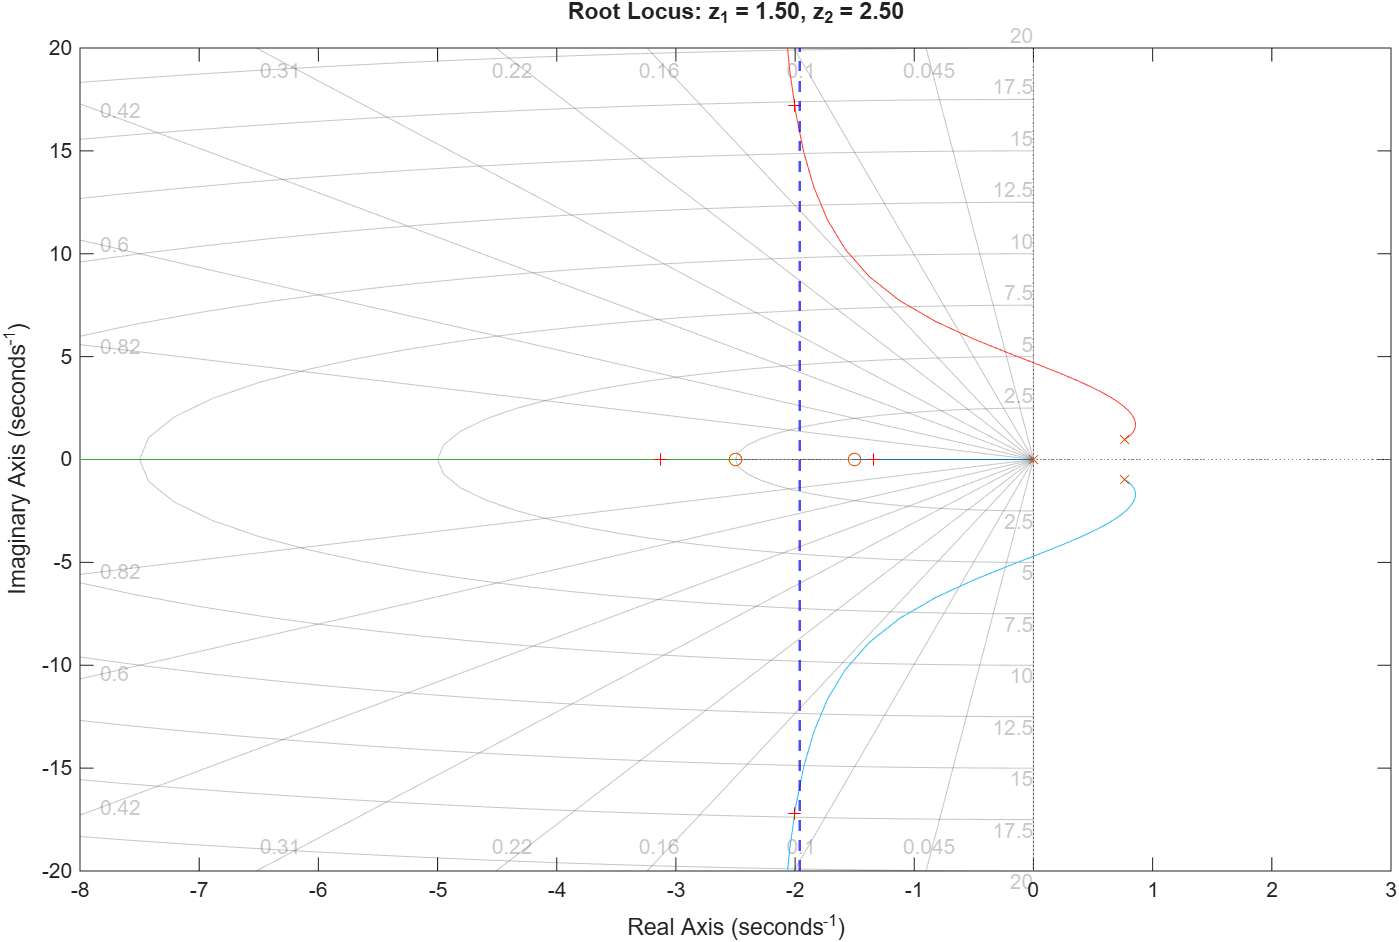
\includegraphics[width=\linewidth]{images/prob2_rlocfind_1.5_2.5.png}
        \caption{Root locus and selected closed-loop poles}
        \label{fig:prob2_rlocfind_1.5_2.5}
    \end{subfigure}
    \hfill
    \begin{subfigure}[t]{0.48\textwidth}
        \centering
        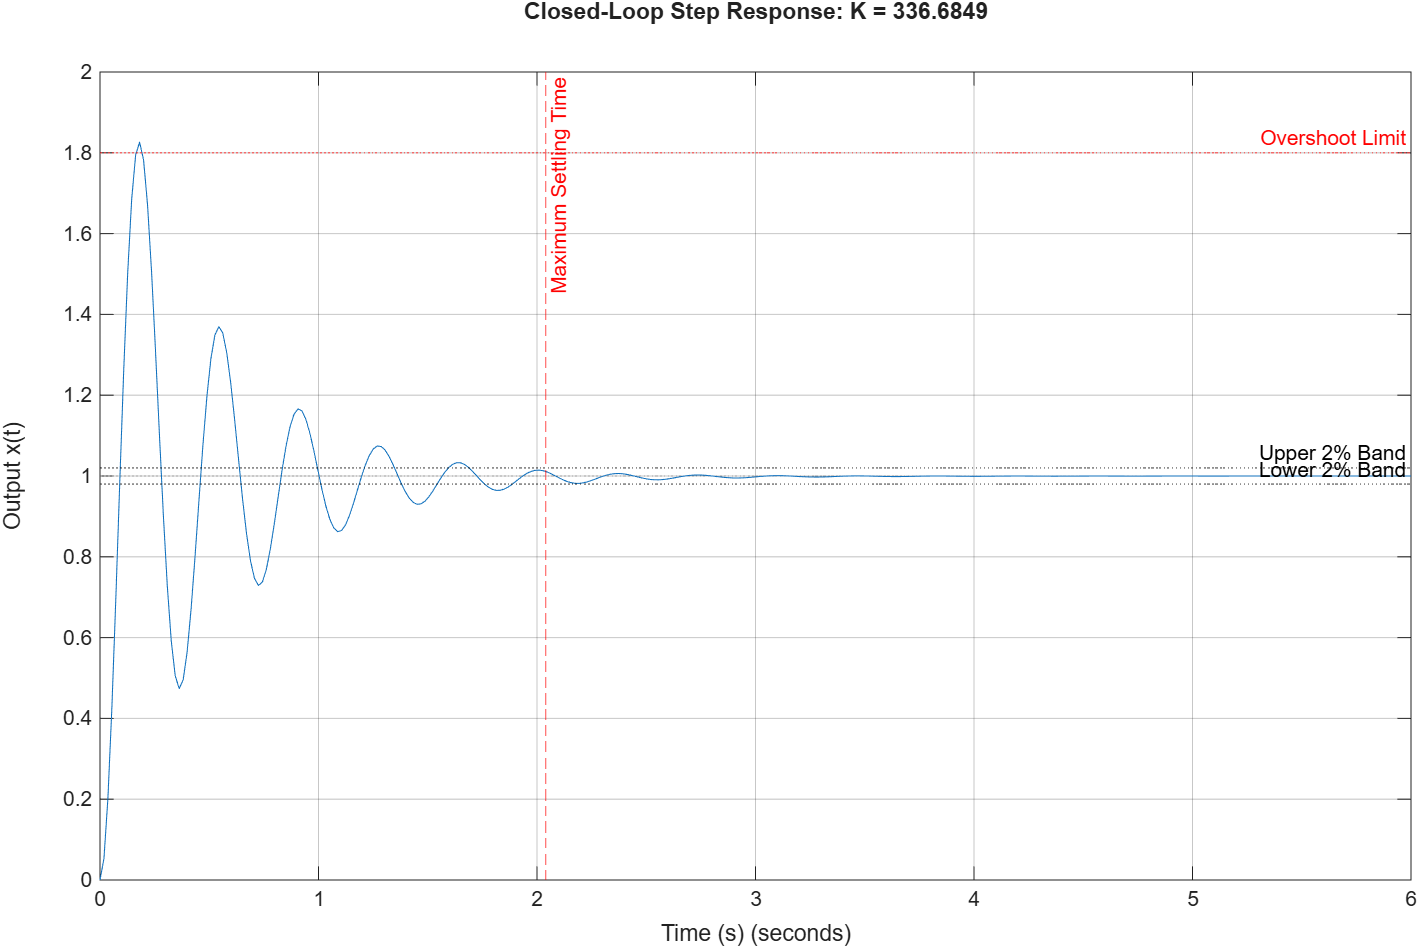
\includegraphics[width=\linewidth]{images/prob2_stepresponse_1.5_2.5.png}
        \caption{Closed-loop step response}
        \label{fig:prob2_stepresponse_1.5_2.5}
    \end{subfigure}
    \caption{PID-controlled system with $z_1=1.5$, $z_2=2.5$ and $p=10$.}
    \label{fig:prob2_pid_1.5_2.5}
\end{figure}

\par\noindent\begin{minipage}{\linewidth}
\begin{lstlisting}[style=outputstyle]
   Selected gain K = 336.6849

    ========== CLOSED-LOOP POLES ==========
    -2.0049 +17.2292i
    -2.0049 -17.2292i
    -3.1290 + 0.0000i
    -1.3411 + 0.0000i

    ========== SPECIFICATION CHECK ==========
    Stable:              1
    Zero step SSE:       1
    DC gain:             1.000000
    Settling time:       1.8869 s (limit 2.04 s)
    Overshoot:           82.64 % (limit 80 %)
\end{lstlisting}
\end{minipage}\par
As expected, a dominant pair of poles with sufficiently negative real components can be realised, and the timing constraint~\ref{spec:settling2} is resultingly met. These dominant poles do not have a sufficiently high damping ratio, and the overshoot constraint~\ref{spec:overshoot2} is not reached. 


This indicates that the magnitude of $z_1$ and $z_2$ should be decreased, such that the centroid of the asymptotic loci is more negative. This will result in the position on these loci where the real component is sufficiently negative having a sufficiently low damping ratio. $z_1=0.5, z_1=1.0$ will have a centroid of $\sigma=\frac{-8.48 +  0.5 + 1.0}{2} = -3.49$. The root loci can be sketched:

\begin{figure}[H]
    \centering
    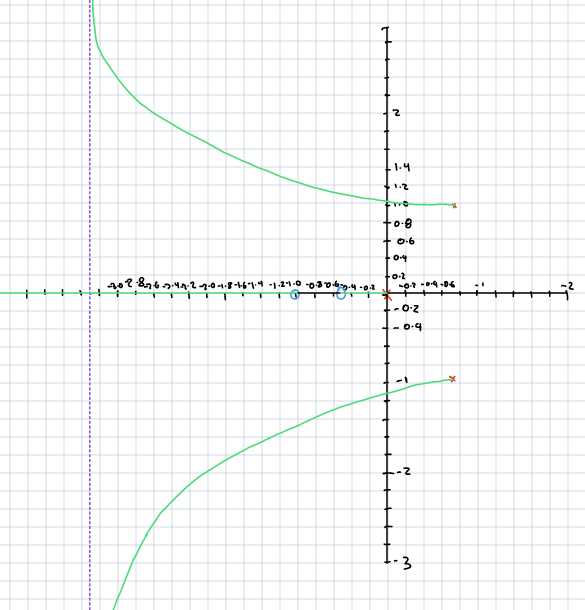
\includegraphics[width=0.8\textwidth]{images/prob2_rootlocussketch_1_0.5.png}
    \caption{Root Locus Sketch for PID-controlled system, $z_1 = 0.5, z_2 = 1.0, p = 10$}
\end{figure}

This topology appears promising for achieving the specification, as a dominant pair of conjugate poles can meet the timing requirement and have a sufficiently high damping ratio (as approximated by a second order model of $\zeta_min$). 

This can be tested using \textit{rlocfind}:
\begin{figure}[H]
    \centering
    \begin{subfigure}[t]{0.48\textwidth}
        \centering
        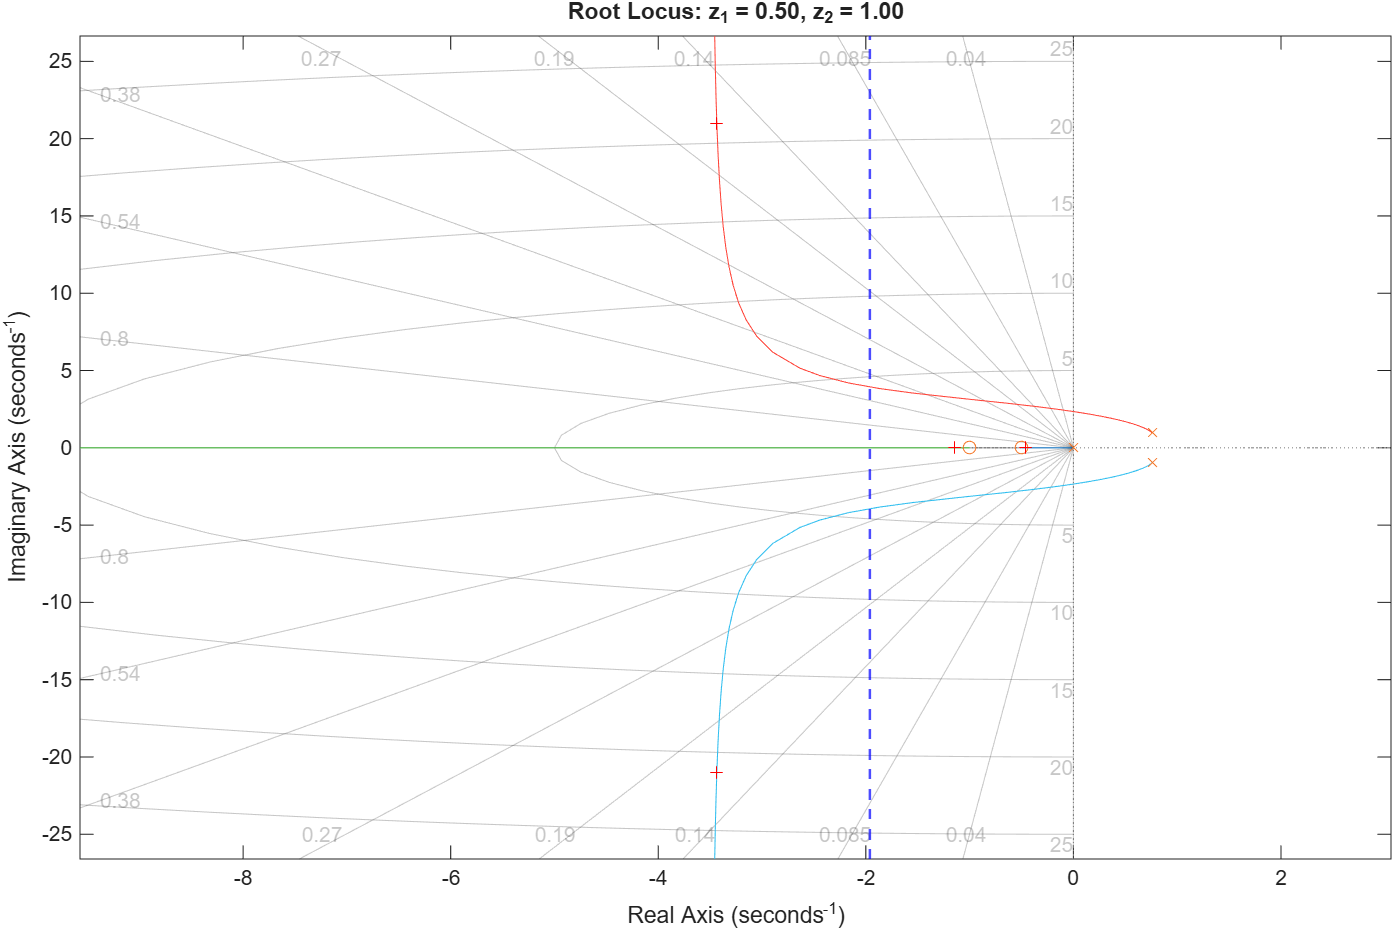
\includegraphics[width=\linewidth]{images/prob2_rlocfind_0.5_1.png}
        \caption{Root locus and selected closed-loop poles}
        \label{fig:prob2_rlocfind_0.5_1}
    \end{subfigure}
    \hfill
    \begin{subfigure}[t]{0.48\textwidth}
        \centering
        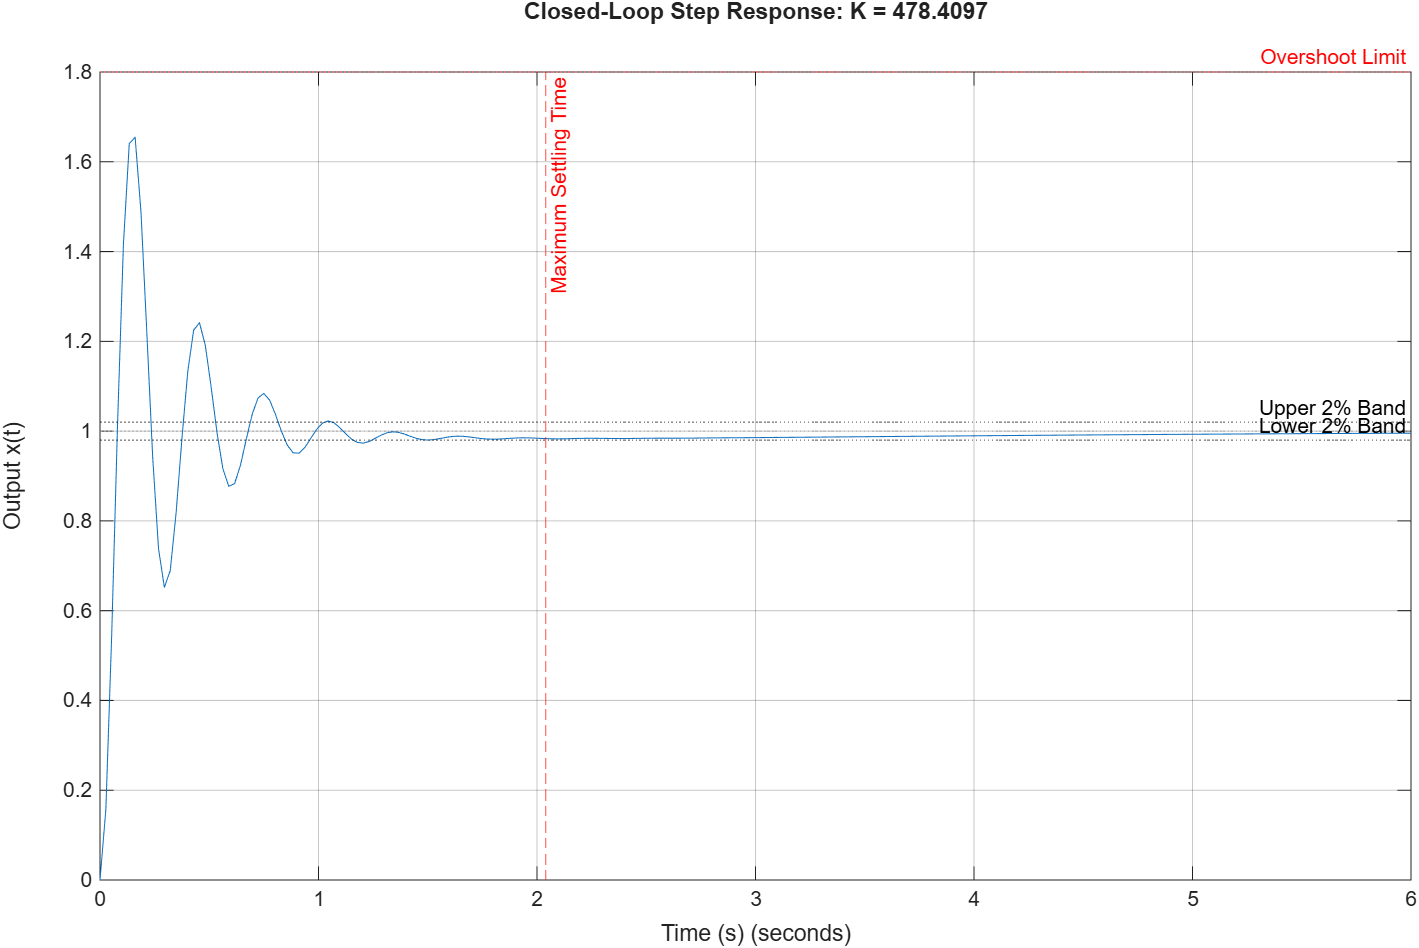
\includegraphics[width=\linewidth]{images/prob2_stepresponse_0.5_1.png}
        \caption{Closed-loop step response}
        \label{fig:prob2_stepresponse_0.5_1}
    \end{subfigure}
    \caption{PID-controlled system with $z_1=0.5$, $z_2=1.0$ and $p=10$.}
    \label{fig:prob2_pid_0.5_1}
\end{figure}
\par\noindent\begin{minipage}{\linewidth}
\begin{lstlisting}[style=outputstyle]
    Selected gain K = 478.4097
    ========== CLOSED-LOOP POLES ==========
    -3.4356 +21.0077i
    -3.4356 -21.0077i
    -1.1496 + 0.0000i
    -0.4592 + 0.0000i


    ========== SPECIFICATION CHECK ==========
    Stable:              1
    Zero step SSE:       1
    DC gain:             1.000000
    Settling time:       1.2443 s (limit 2.04 s)
    Overshoot:           65.43 % (limit 80 %)
\end{lstlisting}
\end{minipage}\par
Using \texttt{rlocfind}, the values of $z_1 = 0.5, z_2 = 1$ with a gain value of $K \approx 478.41$ have yielded a controller meeting the design specifications. The transfer function of this controller is given by:
\begin{equation}
    G_{c}(S) = 478.41 \times \frac{(s+0.5)(s+1)}{s(s+10)} = \underbrace{69.37}_{K_p}+\underbrace{23.92}\frac{1}{s} +\underbrace{40.9s}_{K_d}\frac{1}{\underbrace{0.1}_{T_D}s+1}
    \label{eq:prob2_controller}
\end{equation}
\subsection{Fail-Safe Analysis}
To analyse the failsafe behaviour of this closed loop system, the different failure modes of the controller must first be considered. The failure modes considered in this analysis are:
\begin{itemize}
    \item Partial controller failure, i.e. failure of one of the individual P, I or D actions. The root locus containing the dominant pair of poles for the controller as seen in Fig~\ref{fig:prob2_rlocfind_0.5_1} are seen to cross the real axis and enter the right half plane. This suggests that there exists some $K$ where the system will have poles with positive real components, hence the system will be unstable. To find the scenario where this instability occurs, the values of $K_p, K_i, \& K_d$ can be individually swept from 0\% to 150\% of their nominal values in~\eqref{eq:prob2_controller}, and the overall system stability measured. This can be completed with Matlab, and the critical failure is noted as $K_d \le 3.35$. This will result in an unstable closed loop system as modelled by the linearised plant in~\ref{eq:prob2_linear}, however the behaviour of the non-linear plant may not be that of unbounded oscillation.
    \item Catastrophic controller failure i.e. $f(t)= 0$. In this event, the output of the controller $f(t)$ instantaneously falls to 0. In this case, the expected behaviour of the system is to decay to a stable oscillation, as observed in the initial analysis of this problem. While this is bounded, it represents a non-zero steady state error, and as such will likely imply a non-failsafe system. 
\end{itemize}
Each of these failure modes can be modelled, and the resulting plant behaviour measured. 

\newpage
\begin{thebibliography}{1}
    \bibitem{mathworks:ode45}
    The MathWorks, Inc., ``ode45: Solve nonstiff differential equations---medium order method,''
    \textit{MATLAB Documentation}. Accessed: Oct. 13, 2026. [Online]. Available:
    \url{https://uk.mathworks.com/help/matlab/ref/ode45.html}
\end{thebibliography}

\newpage
\appendix
\section{Matlab Code Listings}

\begin{lstlisting}[
    caption={Matlab code for determining the step response of the closed loop system defined in Problem 1.},
    label={lst:prob1_stepinfo},
]
%% PD Controller with zero at 2.5 and pole at 10
zc = 2.5;
pc = 10;

G_C = tf([1 zc], [1 pc]);

G_CL = G_C * G;

%% Build closed-loop system

T = feedback(K * G_CL, 1);
disp('Step response:')
disp(stepinfo(T))

figure;
step(T);
grid on;

title(sprintf( ...
    'Step Response: z=%.1f, p=%.1f, K=%.2f', ...
    zc, pc, K));


%% Specification checks

fprintf('\n--- Specification checks ---\n');

fprintf('Stable: %d\n', isstable(T));
fprintf('DC gain: %.4f\n', dcgain(T));

info = stepinfo(T);

fprintf('Settling time: %.4f s\n', info.SettlingTime);
fprintf('Overshoot: %.2f %%\n', info.Overshoot);

fprintf('\nClosed-loop poles:\n');
disp(pole(T));

fprintf('Closed-loop zeros:\n');
disp(zero(T));
\end{lstlisting}

\begin{lstlisting}[
    caption={Matlab code for simulating error in estimation of $a_{11}$ and $a_{21}$ in the plant equations.},
    label={lst:prob1_err},
]
\end{lstlisting}

\begin{lstlisting}[
    caption={Matlab code for verifying stability in the case of error in estimation of $a_{11}$ and $a_{21}$ in the plant equations.},
    label={lst:prob1_staberr},
]
\end{lstlisting}
\end{document}
